% Aug 27, 2014: has 118 sections. artisynth.tex and maspack.tex have
%   about 28 and 23 sections, with about 375 words/sec, so we can
%   expect this to be around 45,000 words, or about 120 pages.

\documentclass{article}
\usepackage{amsmath}
\usepackage{framed}
%%
%% Default settings for artisynth
%%
\NeedsTeXFormat{LaTeX2e}
%%\ProvidesPackage{artisynthDoc}[2012/04/05]

\usepackage[T1]{fontenc}
\usepackage[latin1]{inputenc}
\usepackage{listings}
\usepackage{makeidx}
\usepackage{latexml}
\usepackage{graphicx}
\usepackage{framed}
\usepackage{color}

\newcommand{\pubdate}{\today}
\newcommand{\setpubdate}[1]{\renewcommand{\pubdate}{#1}}

\iflatexml
\usepackage{hyperref}
\else
%% then we are making a PDF, so include things that LaTeXML can't handle: 
%% docbook style, \RaggedRight
\usepackage{ifxetex}
\usepackage{pslatex} % fixes fonts; in particular sets a better-fitting \tt font

\usepackage[A4]{artisynth_papersize}
%\usepackage[letter]{artisynth_papersize}
\usepackage[hyperlink]{asciidoc-dblatex} 

%\usepackage{verbatim}
\usepackage{ragged2e}
\setlength{\RaggedRightRightskip}{0pt plus 4em}
\RaggedRight
\renewcommand{\DBKpubdate}{\pubdate}
\renewcommand{\DBKreleaseinfo}{}
\fi

% set hypertext links to be dark blue:
\definecolor{darkblue}{rgb}{0,0,0.8}
\definecolor{sidebar}{rgb}{0.5,0.5,0.7}
\hypersetup{colorlinks=true,urlcolor=darkblue,linkcolor=darkblue}

%%%%%%%%%%%%%%%%%%%%%%%%%%%%%%%%%%%%%%%%%%%%%%%%%%%%%%%%%%%%%%%%%%%%%%%%%%%%%
%
% Define macros for handling javadoc class and method references
%
%%%%%%%%%%%%%%%%%%%%%%%%%%%%%%%%%%%%%%%%%%%%%%%%%%%%%%%%%%%%%%%%%%%%%%%%%%%%%
\makeatletter

% code inspired by http://stackoverflow.com/questions/2457780/latex-apply-an-operation-to-every-character-in-a-string
\def\removeargs #1{\doremoveargs#1$\wholeString\unskip}
\def\doremoveargs#1#2\wholeString{\if#1$%
\else\if#1({()}\else{#1}\taketherest#2\fi\fi}
\def\taketherest#1\fi
{\fi \doremoveargs#1\wholeString}

% Note: still doesn't work properly when called on macro output ...
% i.e., \dottoslash{\concatnames{model}{base}{foo}} fails 
\def\dottoslash #1{\dodottoslash#1$\wholeString\unskip}
\def\dodottoslash#1#2\wholeString{\if#1$%
\else\if#1.{/}\else{#1}\fi\dottaketherest#2\fi}
\def\dottaketherest#1\fi{\fi \dodottoslash#1\wholeString}

% concatenates up to three class/method names together, adding '.' characters
% between them. The first and/or second argument may be empty, in which case
% the '.' is omitted. To check to see if these arguments are empty, we
% use a contruction '\if#1@@', which will return true iff #1 is empty
% (on the assumption that #1 will not contain a '@' character).
\def\concatnames
#1#2#3{\if#1@@\if#2@@#3\else #2.#3\fi\else\if#2@@#1.#3\else#1.#2.#3\fi\fi}

\newcommand{\javabase}{}
\newcommand{\setjavabase}[1]{\renewcommand{\javabase}{#1}}

\iflatexml
\newcommand{\javaclassx}[2][]{%
% Includes code to prevent an extra '.' at the front if #1 is empty. It
% works like this: if '#1' is empty, then '#1.' expands to '.', and so 
% '\if#1..' will return true, in which case we just output '#2'.
\href{@JDOCBEGIN/\concatnames{\javabase}{#1}{#2}@JDOCEND}{#2}}
\newcommand{\javaclass}[2][]{%
\href{@JDOCBEGIN/\concatnames{}{#1}{#2}@JDOCEND}{#2}}

\newcommand{\javamethodArgsx}[2][]{%
\href{@JDOCBEGIN/\concatnames{\javabase}{#1}{#2}@JDOCEND}{#2}}
\newcommand{\javamethodArgs}[2][]{%
\href{@JDOCBEGIN/\concatnames{}{#1}{#2}@JDOCEND}{#2}}
\newcommand{\javamethodAlt}[2]{%
\href{@JDOCBEGIN/\concatnames{}{}{#1}@JDOCEND}{#2}}
\newcommand{\javamethodAltx}[2]{%
\href{@JDOCBEGIN/\concatnames{\javabase}{}{#1}@JDOCEND}{#2}}

\newcommand{\javamethodNoArgsx}[2][]{%
\href{@JDOCBEGIN/\concatnames{\javabase}{#1}{#2}@JDOCEND}{\removeargs{#2}}}
\newcommand{\javamethodNoArgs}[2][]{%
\href{@JDOCBEGIN/\concatnames{}{#1}{#2}@JDOCEND}{\removeargs{#2}}}
\else
\def\javaurl{http://www.artisynth.org/doc/javadocs/}
\newcommand{\javaclassx}[2][]{{\color{darkblue}#2}}
%\href{\javaurl\dottoslash{\concatnames{\javabase}{#1}{#2}}.html}{#2}}
\newcommand{\javamethodArgsx}[2][]{{\color{darkblue}#2}}
\newcommand{\javamethodNoArgsx}[2][]{{\color{darkblue}\removeargs{#2}}}
\newcommand{\javaclass}[2][]{{\color{darkblue}#2}}
%\href{\javaurl\dottoslash{\concatnames{\javabase}{#1}{#2}}.html}{#2}}
\newcommand{\javamethodArgs}[2][]{{\color{darkblue}#2}}
\newcommand{\javamethodNoArgs}[2][]{{\color{darkblue}\removeargs{#2}}}
\newcommand{\javamethodAlt}[2]{{\color{darkblue}{#2}}}
\newcommand{\javamethodAltx}[2]{{\color{darkblue}{#2}}}
\fi

\newcommand{\javamethod}{\@ifstar\javamethodNoArgs\javamethodArgs}
\newcommand{\javamethodx}{\@ifstar\javamethodNoArgsx\javamethodArgsx}

%%%%%%%%%%%%%%%%%%%%%%%%%%%%%%%%%%%%%%%%%%%%%%%%%%%%%%%%%%%%%%%%%%%%%%%%%%%%%
%
% Define macros for sidebars
%
%%%%%%%%%%%%%%%%%%%%%%%%%%%%%%%%%%%%%%%%%%%%%%%%%%%%%%%%%%%%%%%%%%%%%%%%%%%%%

\iflatexml
\newenvironment{sideblock}{\begin{quote}}{\end{quote}}
\else
\usepackage[strict]{changepage}
\definecolor{sidebarshade}{rgb}{1.0,0.97,0.8}
\newenvironment{sideblock}{%
    \def\FrameCommand{%
    \hspace{1pt}%
    {\color{sidebar}\vrule width 2pt}%
    %{\vrule width 2pt}%
    {\color{sidebarshade}\vrule width 4pt}%
    \colorbox{sidebarshade}%
  }%
  \MakeFramed{\advance\hsize-\width\FrameRestore}%
  \noindent\hspace{-4.55pt}% disable indenting first paragraph
  \begin{adjustwidth}{}{7pt}%
  %\vspace{2pt}\vspace{2pt}%
}
{%
  \vspace{2pt}\end{adjustwidth}\endMakeFramed%
}
\fi

\iflatexml
\newenvironment{shadedregion}{%
  \definecolor{shadecolor}{rgb}{0.96,0.96,0.98}%
  \begin{shaded*}%
% Put text inside a quote to create a surrounding blockquote that
% will properly accept the color and padding attributes
  \begin{quote}%
}
{%
  \end{quote}%
  \end{shaded*}%
}
\else
\newenvironment{shadedregion}{%
  \definecolor{shadecolor}{rgb}{0.96,0.96,0.98}%
  \begin{shaded*}%
}
{%
  \end{shaded*}%
}
\fi

% Wanted to create a 'listing' environment because lstlisting is
% tedious to type and because under latexml it may need
% some massaging to get it to work properly. But hard to do
% because of the verbatim nature of listing
%\iflatexml
%\newenvironment{listing}{\begin{lstlisting}}{\end{lstlisting}}%
%\else
%\newenvironment{listing}{\begin{lstlisting}}{\end{lstlisting}}%
%\fi

\iflatexml\else
% fancyhdr was complaining that it wanted a 36pt header height ...
\setlength{\headheight}{36pt}
\fi

% abbreviation for backslash character
\newcommand\BKS{\textbackslash}


% Convenience stuff
\newcommand{\ifLaTeXMLelse}[2]{%
  \iflatexml %
  #1 %
  \else %
  #2 %
  \fi %
}

\newcommand{\ifLaTeXML}[1]{ %
  \iflatexml %
  #1 %
  \fi %
}

\makeatother

\def\matl{\left(\begin{matrix}}
\def\matr{\end{matrix}\right)}

\def\Bthe{\boldsymbol\theta}
\def\Bom{\boldsymbol\omega}
\def\Bdel{\boldsymbol\delta}
\def\Blam{\boldsymbol\lambda}
\def\Bphi{\boldsymbol\phi}
\def\Bxi{\boldsymbol\xi}
\def\Bgam{\boldsymbol\gamma}
\def\Bsig{\boldsymbol\sigma}
\def\Bnu{\boldsymbol\nu}
\def\Bmu{\boldsymbol\mu}

\def\A{{\bf A}}
\def\B{{\bf B}}
\def\C{{\bf C}}
\def\D{{\bf D}}
\def\G{{\bf G}}
\def\H{{\bf H}}
\def\I{{\bf I}}
\def\J{{\bf J}}
\def\K{{\bf K}}
\def\Jc{{\bf J}_c}
\def\L{{\bf L}}
\def\M{{\bf M}}
\def\N{{\bf N}}
\def\O{{\bf O}}
\def\P{{\bf P}}
\def\Q{{\bf Q}}
\def\R{{\bf R}}
\def\T{{\bf T}}
\def\U{{\bf U}}
\def\W{{\bf W}}
\def\X{{\bf X}}
\def\Minv{{\bf M}^{-1}}

\def\a{{\bf a}}
\def\b{{\bf b}}
\def\c{{\bf c}}
\def\d{{\bf d}}
\def\e{{\bf e}}
\def\f{{\bf f}}
\def\g{{\bf g}}
\def\l{{\bf l}}
\def\m{{\bf m}}
\def\n{{\bf n}}
\def\p{{\bf p}}
\def\q{{\bf q}}
\def\u{{\bf u}}
\def\v{{\bf v}}
\def\w{{\bf w}}
\def\x{{\bf x}}
\def\y{{\bf y}}
\def\z{{\bf z}}

\def\ma{{\bf m}_\alpha}
\def\mb{{\bf m}_\beta}
\def\va{{\bf v}_\alpha}
\def\vb{{\bf v}_\beta}
\def\vp{{\bf v}_\rho}
\def\vk{{\bf v}_k}
\def\ua{{\bf u}_\alpha}
\def\ub{{\bf u}_\beta}
\def\uk{{\bf u}_k}
\def\uj{{\bf u}_j}
\def\mar{{\bf m}_{\alpha r}}
\def\mbr{{\bf m}_{\beta r}}

\def\Maa{{\bf M}_{\alpha\alpha}}
\def\Mab{{\bf M}_{\alpha\beta}}
\def\Mba{{\bf M}_{\beta\alpha}}
\def\Mbb{{\bf M}_{\beta\beta}}
\def\hatMaa{\hat{\bf M}_{\alpha\alpha}}
\def\hatMab{\hat{\bf M}_{\alpha\beta}}
\def\hatMba{\hat{\bf M}_{\beta\alpha}}
\def\hatMbb{\hat{\bf M}_{\beta\beta}}
\def\Mbp{{\bf M}_{\beta\rho}}
\def\Map{{\bf M}_{\alpha\rho}}
\def\Mpa{{\bf M}_{\rho\alpha}}
\def\Mpb{{\bf M}_{\rho\beta}}
\def\Mpp{{\bf M}_{\rho\rho}}
\def\Mbk{{\bf M}_{\beta k}}
\def\Mak{{\bf M}_{\alpha k}}
\def\Mka{{\bf M}_{k\alpha}}
\def\Mkb{{\bf M}_{k\beta}}
\def\Mkk{{\bf M}_{kk}}

\def\Ga{{\bf G}_{\alpha}}
\def\Gp{{\bf G}_{\rho}}
\def\Gaa{{\bf G}_{\alpha\alpha}}
\def\Gab{{\bf G}_{\alpha\beta}}
\def\Gba{{\bf G}_{\beta\alpha}}
\def\Gbb{{\bf G}_{\beta\beta}}
\def\Gap{{\bf G}_{\alpha\rho}}
\def\Gpa{{\bf G}_{\rho\alpha}}
\def\Gbp{{\bf G}_{\beta\rho}}
\def\Gak{{\bf G}_{\alpha k}}
\def\Gka{{\bf G}_{k\alpha}}
\def\Gja{{\bf G}_{j\alpha}}
\def\Gkb{{\bf G}_{k\beta}}
\def\Gbk{{\bf G}_{\beta k}}

\def\lama{\Blam_{\alpha}}
\def\lamb{\Blam_{\beta}}
\def\lamp{\Blam_{\rho}}
\def\lamk{\Blam_{k}}
\def\lams{\Blam_{\sigma}}

\def\ba{{\bf b}_{\alpha}}
\def\bb{{\bf b}_{\beta}}
\def\fp{{\bf f}_{\rho}}
\def\fa{{\bf f}_{\alpha}}
\def\qa{{\bf q}_{\alpha}}
\def\qb{{\bf q}_{\beta}}
\def\za{{\bf z}_{\alpha}}
\def\zb{{\bf z}_{\beta}}
\def\wa{{\bf w}_{\alpha}}
\def\wb{{\bf w}_{\beta}}

\def\Na{\bar{\bf N}_{\alpha}}
\def\Nb{\bar{\bf N}_{\beta}}

\def\Up{{\bf U}_p}
\def\Un{{\bf U}_n}

\def\dFdl{\frac{\partial F}{\partial l}}
\def\dFddl{\frac{\partial F}{\partial \dot l}}



\setcounter{tocdepth}{5}
\setcounter{secnumdepth}{3}

\title{ArtiSynth Modeling Guide}
\author{John Lloyd and Antonio S\'anchez}
\setpubdate{September 15, 2014}
\iflatexml
\date{}
\fi

\begin{document}

\maketitle

\iflatexml{\large\pubdate}\fi

\tableofcontents

\setjavabase{artisynth.core.modelbase}

% basic links to other docs: http://www.artisynth.org/doc/html/xxx/xxx.html#sec

\section{Introduction}

This guide describes how to create mechanical and biomechanical models
in ArtiSynth using its Java API. 

It is assumed that the reader is familiar with basic Java programming,
including variable assignment, control flow, exceptions, functions and
methods, object construction, inheritance, and method overloading.
Some familiarity with the {\tt Collections} packages in {\tt
java.util}, such as {\tt ArrayList} and {\tt LinkedList} is also
useful.

\subsection{How to read this guide}

Section \ref{Overview:sec} offers a general overview of ArtiSynth's
software design, and briefly describes the algorithms used for
physical simulation (Section \ref{PhysicsSimulation:sec}). The latter
section may be skipped on first reading. A more comprehensive
\href{http://www.artisynth.org/doc/artisynth.pdf}{overview paper} is
available online.

The remainder of the manual gives details instructions on how to build
various types of mechanical and biomechanical models.  Sections
\ref{MechModelsI:sec} and \ref{MechModelsII:sec} give detailed
information about building general mechanical models, involving
particles, springs, rigid bodies, joints, constraints, and
contact. Section \ref{SimulationControl:sec} describes how to add control panels,
controllers, and input and output data streams to a simulation.
Section \ref{FEMModels:sec} describes how to incorporate finite
element models.

If time permits, the reader will profit from a top-to-bottom read.
However, this may not always be necessary. Many of the sections
contain detailed demonstration examples, all of which are available in
the package {\tt artisynth.demos.tutorial} and which may be run from
ArtiSynth using model menu {\sf Models > All demos > tutorials}.  The
More experienced readers may wish to find an appropriate example and
then work backwards into the text and preceeding section for any
needed explanatory detail.

\section{ArtiSynth Overview}
\label{Overview:sec}

ArtiSynth is an open-source, Java-based system for creating and
simulating mechanical and biomechanical models, with specific
capabilities for the combined simulation of rigid and deformable
bodies, together with contact and constraints. It is presently
directed at application domains in biomechanics, medicine, physiology,
and dentistry, but it can also be applied to other areas such as
traditional mechanical simulation, ergonomic design, and graphical and
visual effects.

\subsection{System structure}

An ArtiSynth model is composed of a hierarchy of models and model
components (Figure ref{components:fig}) which are implemented by
various Java classes. These may include sub-models (including finite
element models), particles, rigid bodies, springs, connectors, and
constraints.  The component hierarchy may be in turn connected to
various {\it agent} components, such as control panels, controllers
and monitors, and input and output data streams (i.e., {\it probes}),
which have the ability to control and record the simulation as it
advances in time. Agents are presented in more detail in Section
\ref{SimulationControl:sec}. 

The models and agents are collected together within a top-level
component known as a {\it root model}.  Simulation proceeds under the
control of a {\it scheduler}, which advances the models through time
using a physics simulator. A rich graphical user interface (GUI)
allows users to view and edit the model hierarchy, modify component
properties, and edit and temporally arrange the input and output
probes using a {\it timeline} display.

\subsubsection{Model components}

Every ArtiSynth component is an instance of
\javaclass[artisynth.core.modelbase]{ModelComponent}. When connected
to the hierarchy, it is assigned a unique number relative to its
parent; the parent and number can be obtained using the methods
\javamethod[artisynth.core.modelbase.ModelComponent]{getParent()} and
\javamethod[artisynth.core.modelbase.ModelComponent]{getNumber()},
respectively.  Components may also be assigned a name (using
\javamethod*[artisynth.core.modelbase.ModelComponent]{setName()})
which is then returned using
\javamethod*[artisynth.core.modelbase.ModelComponent]{getName()}.

A sub-interface of {\tt ModelComponent} includes
\javaclass[artisynth.core.modelbase]{CompositeComponent}, which
contains child components.  A
\javaclass[artisynth.core.modelbase]{ComponentList} is a {\tt
CompositeComponent} which simply contains a list of other components
(such as particles, rigid bodies, sub-models, etc.).

Components which contain state information (such as position and
velocity) should extend {\tt HasState}, which provides
the methods
\javamethod*[artisynth.core.modelbase.HasState]{getState()}
and
\javamethod*[artisynth.core.modelbase.HasState]{setState()}
for saving and restoring state.

A {\tt Model} is a sub-interface of {\tt CompositeComponent} and {\tt
HasState} that contains the notion of advancing through time and which
implements this with the methods {\tt initialize(t0)} and {\tt
advance(t0, t1, flags)}. The most common instance of {\tt Model} used
in ArtiSynth is {\tt MechModel} (Section \ref{MechModel:sec}), which
is the top-level container for a mechanical or biomechanical model.

\subsubsection{The RootModel}
\label{RootModel:sec}

The top-level component in the hierarchy is the root model, which is a
subclass of \javaclass[artisynth.core.workspace]{RootModel} and
which contains a list of models along with lists of agents used to
control and interact with these models. The component lists in {\tt
RootModel} include:

\begin{shadedregion}
\begin{tabular}{ll}
\tt models & top-level models of the component hierarchy \\
\tt inputProbes & input data streams for controlling the simulation \\
\tt controllers & functions for controlling the simulation \\
\tt monitors & functions for observing the simulation \\
\tt outputProbes & output data streams for observing the simulation \\
\end{tabular}
\end{shadedregion}

Each agent may be associated with a specific top-level model.

\subsubsection{Component path names}
\label{PathNames:sec}

The names and/or numbers of a component and its ancestors can be used to
form a component path name. This path has a construction 
analogous to Unix file path names, with the '/' character acting as a
separator. Absolute paths start with '/', which indicates the root
model. Relative paths omit the leading '/' and can begin lower down
in the hierarchy. A typical path name might be
\begin{verbatim}
  /models/JawHyoidModel/axialSprings/lad
\end{verbatim}
For nameless components in the path, their numbers can be used
instead.  Numbers can also be used for components that have
names. Hence the path above could also be represented using
only numbers, as in
\begin{verbatim}
  /0/0/1/5
\end{verbatim}
although this would most likely appear only in machine-generated
output.

\subsubsection{Model advancement}

ArtiSynth simulation proceeds by advancing all of the root model's
top-level models through a sequence of time steps. Every time
step is achieved by calling each model's 
\javamethod*[artisynth.core.modelbase.Model]{advance()} method:
\begin{lstlisting}[]
  public StepAdjustment advance (double t0, double t1) {
     ... perform simulation ...
  }
\end{lstlisting}
This method advances the model from time {\tt t0} to time {\tt t1},
performing whatever physical simulation is required (see Section
\ref{PhysicsSimulation:sec}). The method may optionally return a {\tt
StepAdjusment} indicating that the step size ({\tt t1} - {\tt t0}) was
too large and that the advance should be redone with a smaller step
size. 

The root model has it's own
\javamethod*[artisynth.core.workspace.RootModel]{advance()}, which in
turn calls the advance method for all of the top-level models, in
sequence. The advance of each model is surrounded by the application
whatever agents are associated with that model. This is done
by calling the agent's {\tt apply()} method:
\begin{lstlisting}[]
   model.preadvance (t0, t1);
   for (each input probe p) {
      p.apply (t1);
   }
   for (each controller c) {
      c.apply (t0, t1);
   }
   model.advance (t0, t1);
   for (each monitor m) {
      m.apply (t0, t1);
   }
   for (each output probe p) {
      p.apply (t1);
   }
\end{lstlisting}
Agents not associated with a specific model are applied by the root
model's {\tt advance()} method before (or after) the advance of all
other models.

More precise details about model advancement are given in the 
\href{http://www.artisynth.org/doc/html/artisynth/artisynth.html}{
ArtiSynth Reference Manual}.

\subsubsection{MechModel}
\label{MechModel:sec}

Most ArtiSynth applications contain a single top-level model which is
an instance of \javaclass[artisynth.core.mechmodels]{MechModel}.  This
is a \javaclass[artisynth.core.modelbase]{CompositeComponent} that may
(recursively) contain an arbitrary number of mechanical components,
including finite element models, other {\tt MechModel}s, particles,
rigid bodies, constraints, attachments, and various force effectors.
The {\tt MechModel} {\tt advance()} method invokes a physics simulator
that advances these components forward in time (Section
\ref{PhysicsSimulation:sec}).

For convenience each {\tt MechModel} contains a number of predefined
containers for different component types, including:

%\begin{framed}%
%\colorbox{shadecolor}{%
\begin{shadedregion}
\begin{tabular}{ll}
\tt particles & 3 DOF particles \\
\tt rigidBodies & 6 DOF rigid bodies \\
\tt axialSprings & point-to-point springs \\
\tt connectors & joint-type connectors between bodies \\
\tt constrainers & general constraints \\
\tt forceEffectors & general force-effectors \\
\tt attachments & attachments between dynamic components \\
\tt renderables & renderable components (for visualization only) \\
\end{tabular}
\end{shadedregion}
Each of these is a child component of {\tt MechModel} and is
implemented as a
\javaclass[artisynth.core.modelbase]{ComponentList}. Special methods
are provided for adding and removing items from them. However,
applications are not required to use these containers, and may instead
create any component containment structure that is appropriate
(Section \ref{GeneralArrangements:sec}).  If not used, the containers
will simply remain empty.

\subsection{Physics simulation}
\label{PhysicsSimulation:sec}

Only a brief summary of ArtiSynth physics simulation is described
here.  Full details are given in \cite{lloyd2012artisynth} and in the
related
\href{http://www.artisynth.org/doc/artisynth.pdf}{overview
paper}.

For purposes of physics simulation, the components of a {\tt
MechModel} are grouped as follows:

\begin{description}
	
\item[Dynamic components] \mbox{}\hfill\\ Components, such as a
particles and rigid bodies, that contain position and velocity state,
as well as mass. All dynamic components are instances of
the Java interface
\javaclass[artisynth.core.mechmodels]{DynamicComponent}.

\item[Force effectors] \mbox{}\hfill\\
Components, such as springs or finite elements,
that exert forces between dynamic components.
All force effectors are instances of the Java interface
\javaclass[artisynth.core.mechmodels]{ForceEffector}.

\item[Constrainers] \mbox{}\hfill\\
Components that enforce constraints between dynamic components. 
All constrainers are instances of the Java interface
\javaclass[artisynth.core.mechmodels]{Constrainer}.

\item[Attachments] \mbox{}\hfill\\
Attachments between dynamic components. While technically these
are constraints, they are implemented using a different approach.
All attachment components are instances of
\javaclass[artisynth.core.mechmodels]{DynamicAttachment}.

\end{description}

The positions, velocities, and forces associated with all the
dynamic components are denoted by the composite vectors 
$\q$, $\u$, and $\f$. 
In addition, the composite mass matrx is given by
$\M$. 
Newton's second law then gives
\begin{equation}
\f = \frac{d \M \u}{d t} = \M \dot\u + \dot\M \u,
\label{newton:eqn}
\end{equation}
%
where the $\dot\M \u$ accounts for various ``fictitous'' forces.

Each integration step involves solving for
the velocities $\u^{k+1}$ at time step $k+1$ given the velocities and forces
at step $k$. One way to do this is to solve the expression
%
\begin{equation}
\M \, \u^{k+1} = \M \u^k + h \bar\f
\label{velupdate:eqn}
\end{equation}
%
for $\u^{k+1}$, where $h$ is the step size and 
$\bar\f \equiv \f - \dot\M \u$. Given the updated velocities $\u^{k+1}$, one can
determine $\dot\q^{k+1}$ from
%
\begin{equation}
\dot\q^{k+1} = \Q \u^{k+1},
\end{equation}
%
where $\Q$ accounts for situations (like rigid bodies) where $\dot\q \ne
\u$, and then solve for the updated positions using 
%
\begin{equation}
\q^{k+1} = \q^k + h \dot \q^{k+1}.
\label{posupdate:eqn}
\end{equation}
%
(\ref{velupdate:eqn}) and (\ref{posupdate:eqn}) together comprise a
simple {\it symplectic Euler} integrator.

In addition to forces, bilateral and unilateral constraints give rise to
locally linear constraints on $\u$ of the form
\begin{equation}
\G(\q) \u = 0, \qquad \N(\q) \u \ge 0.
\label{constraints:eqn}
\end{equation}
%
Bilateral constraints may include rigid body joints, FEM
incompressibility, and point-surface constraints, while unilateral
constraints include contact and joint limits.  Constraints give rise
to constraint forces (in the directions $\G(\q)^T$ and $\N(\q)^T$)
which supplement the forces of (\ref{newton:eqn}) in order to enforce
the constraint conditions.  In addition, for unilateral constraints,
we have a complementarity condition in which $\N \u > 0$ implies no
constraint force, and a constraint force implies $\N \u = 0$.  Any
given constraint usually involves only a few dynamic components and so
$\G$ and $\N$ are generally sparse.

Adding constraints to the velocity solve (\ref{velupdate:eqn})
leads to a mixed linear complementarity problem (MLCP)
of the form
\begin{gather}
\left(
\begin{matrix}
\hat\M^{k} & -\G^{T} & -\N^{T} \\
\G & 0 & 0 \\
\N & 0 & 0 
\end{matrix}
\right)
\left(
\begin{matrix}
\u^{k+1} \\
\Blam \\
\z
\end{matrix}
\right)
+
\left(
\begin{matrix}
-\M \u^{k} - h \hat\f^{k} \\
-\g^k \\
-\n^k
\end{matrix}
\right)
=
\left(
\begin{matrix}
0 \\
0 \\
\w
\end{matrix}
\right), \notag \\
0 \le \z \perp \w \ge 0,
\label{KKTvelocity:eqn}
\end{gather}
where $\w$ is a slack variable, $\Blam$ and $\z$ give the force
constraint impulses over the time step, $\g$ and $\n$ are derivative
terms arising if $\G$ and $\N$ are time varying.  In addition,
$\hat\M$ and $\hat\f$ are $\M$ and $\bar\f$ augmented with stiffness
and damping terms terms to accommodate implicit integration, which
is often required for problems involving deformable bodies.

Attachments can be implemented by constraining the velocities of
the attached components using special constraints of the form
%
\begin{equation}
\u_j = -\G_{j\alpha} \u_\alpha
\label{attachments:eqn}
\end{equation}
%
where $\u_j$ and $\u_\alpha$ denote velocities of the attached and
non-attached components. These constraints could be added directly to
(\ref{KKTvelocity:eqn}), but their special form allows us to
explicitly solve for $\u_j$, and hence actually simplify
(\ref{KKTvelocity:eqn}), by factoring out the attached velocities
before solution.

The MLCP (\ref{KKTvelocity:eqn}) corresponds to a single step
integrator. However, higher order integrators, such as Newmark
methods, usually give rise to MLCPs with an equivalent form.  Most
ArtiSynth integrators use some variation of (\ref{KKTvelocity:eqn}) to
determine the system velocity at each time step.

To set up (\ref{KKTvelocity:eqn}), the {\tt MechModel} component
hierarchy is traversed and the methods of the different component
types are queried for the required values.  Dynamic compoinents (type
{\tt DynamicComponent}) provide $\q$, $\u$, and $\M$; force effectors
({\tt ForceEffector}) determine $\hat\f$ and the stiffness/damping
augmentation used to produce $\hat\M$; constrainers ({\tt
Constrainer}) supply $\G$, $\N$, $\g$ and $\n$, and attachments ({\tt
DynamicAttachment}) provide the information needed to factor out
attached velocities.

\subsection{Basic packages}

The core code of the ArtiSynth project is divided into three main
packages, each with a number of sub-packages.

\subsubsection{maspack}

The packages under {\tt maspack} contain general computational
utilities that are independent of ArtiSynth and could be
used in variety of other contexts. The main packages are:

\begin{lstlisting}[]
maspack.util               // general utilities
maspack.matrix             // matrix and linear algebra
maspack.graph              // graph algorithms
maspack.fileutil           // remote file access 
maspack.properties         // property implementation
maspack.spatialmotion      // 3D spatial motion and dynamics
maspack.solvers            // LCP solvers and linear solver interfaces
maspack.render             // viewer and rendering classes
maspack.geometry           // 3D geometry and meshes
maspack.collision          // collision detection
maspack.widgets            // Java swing widgets for maspack data types 
maspack.apps               // stand-alone programs based only on maspack
\end{lstlisting}

\subsubsection{artisynth.core}

The packages under {\tt artisynth.core} contain the core code for
ArtiSynth model components and it's GUI infrastructure.

\begin{lstlisting}[]
artisynth.core.util        // general ArtiSynth utilities
artisynth.core.modelbase   // base classes for model components
artisynth.core.materials   // materials for springs and finite elements
artisynth.core.mechmodels  // basic mechanical models
artisynth.core.femmodels   // finite element models
artisynth.core.probes      // input and output probes
artisynth.core.workspace   // RootModel and associated components
artisynth.core.driver      // start ArtiSynth and drive the simulation
artisynth.core.gui         // graphical interface
artisynth.core.inverse     // inverse controller
\end{lstlisting}

\subsubsection{artisynth.demos}

These packages contain demonstration models that illustrate
ArtiSynth's modeling capabilities:

\begin{lstlisting}[]
artisynth.demos.mech       // mechanical model demos
artisynth.demos.fem        // demos involving finite elements
artisynth.demos.inverse    // demos involving inverse control
artisynth.demos.tutorial   // demos in this manual
\end{lstlisting}

\subsection{Properties}
\label{Properties:sec}

ArtiSynth components expose {\it properties}, which provide a uniform
interface for accessing their internal parameters and
state. Properties vary from component to component; those for {\tt
RigidBody} include {\tt position}, {\tt orientation}, {\tt mass}, and
{\tt density}, while those for {\tt AxialSpring} include {\tt
restLength} and {\tt material}. Properties are particularly
useful for automatically creating control panels and
probes, as described in Section \ref{SimulationControl:sec}.
They are also used for automating component serialization.

Properties are described only briefly in this section; 
more detailed descriptions are available in the
\href{http://www.artisynth.org/doc/html/maspack/maspack.html}{
Maspack Reference Manual} and the 
\href{http://www.artisynth.org/doc/artisynth.pdf}{overview
paper}.

The set of properties defined for a component is fixed for that
component's class; while property values may vary between component
instances, their definitions are class-specific.  
Properties are exposed by a class through code contained in the class
definition, as described in Section \ref{CustomProperties:sec}.

\subsubsection{Property handles and paths}

Each property has a unique name which may be used to obtain a {\it
property handle} through which the property's value may be queried or
set for a particular component. Property handles are implemented by
the class \javaclass[maspack.property]{Property} and are returned by
the component's
\javamethod*[maspack.properties.HasProperties]{getProperty()} method.
{\tt getProperty()} takes a property's name and returns the
corresponding handle. For example, components of type {\tt Muscle}
have a property {\tt excitation}, for which a handle
may be obtained using a code fragment such as
\begin{lstlisting}[]
  Muscle muscle; 
  ...
  Property prop = muscle.getProperty ("excitation");
\end{lstlisting}
Property handles can also be obtained for
sub-components, using a {\it property path} that consists
of a path to the sub-component followed by a
``{\tt :}'' and the property name. For example,
to obtain the {\tt excitation} property for a sub-component
located by {\tt axialSprings/lad} relative to a {\tt MechModel},
once could use a call of the form
\begin{lstlisting}[]
  MechModel mechMod;
  ...
  Property prop = mechMod.getProperty ("axialSprings/lad:excitation");
\end{lstlisting}

\subsubsection{Composite and inheritable properties}
\label{CompositeInheritableProperties:sec}

\begin{figure}[t]
\begin{center}
 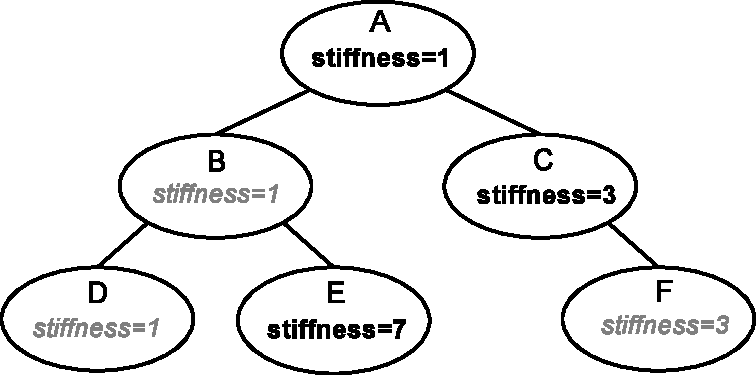
\includegraphics[width=3.75in]{images/inheritedProperties}
\end{center}
\caption{Inheritance of a property named {\it stiffness} among
a component hierarchy. Explicit settings are in bold; inherited settings
are in gray italic.}
\label{inheritedProperties:fig}
\end{figure}

Composite properties are possible, in which a property value is a
composite object that in turn has sub-properties. A good example of
this is the {\tt RenderProps} class, which is
associated with the property {\tt renderProps} for renderable objects
and which itself can have a number of sub-properties such as {\tt
visible}, {\tt faceStyle}, {\tt faceColor}, {\tt lineStyle}, {\tt
lineColor}, etc.

Properties can be declared to be {\tt inheritable}, so that their
values can be inherited from the same properties hosted by ancestor
components further up the component hierarchy. Inheritable properties
require a more elaborate declaration and are associated with a {\it
mode} which may be either {\tt Explicit} or {\tt Inherited}.  If a
property's mode is inherited, then its value is obtained from
the closest ancestor exposing the same property whose mode is
explicit. In Figure (\ref{inheritedProperties:fig}), the property {\it
stiffness} is explicitly set in components A, C, and E, and inherited
in B and D (which inherit from A) and F (which inherits from C).

\subsection{Creating an application model}
\label{CreatingAnApplication:sec}

ArtiSynth applications are created by writing and compiling
an {\it application model} that is a subclass of {\tt RootModel}.
This application-specific root model is then loaded and run by the
ArtiSynth program.

The code for the application model should:

\begin{itemize}

\item Declare a no-args constructor

\item Override the {\tt RootModel}
\javamethod*[artisynth.core.workspace.RootModel]{build()}
method to construct the application.

\end{itemize}

ArtiSynth can load a model either using the build method
or by reading it from a file:

\begin{description}

\item[Build method] \mbox{}

ArtiSynth creates an instance of the
model using the no-args constructor, assigns it a name
(which is either user-specified or the simple name of the class), and
then calls the {\tt build()} method to perform the actual
construction.

\item[Reading from a file] \mbox{}

ArtiSynth creates an instance of the
model using the no-args constructor, and then the model is named
and constructed by reading the file.

\end{description}

The no-args constructor should perform whatever initialization is
required in both cases, while the {\tt build()} takes the place of the
file specification. Unless a model is originally created using a file
specification (which is tedious at the present time), the first time
creation of a model will almost always entail using the {\tt build()}
method.

The general template for application model code looks like this:

\begin{lstlisting}[]
package artisynth.models.experimental; // package where the model resides
import artisynth.core.workspace.RootModel;
... other imports ...

public class MyModel extends RootModel {

   // no-args constructor
   public MyModel() {
      ... basic initialization ...
   }

   // build method to do model construction
   public void build (String[] args) {
      ... code to build the model ....
   }
}
\end{lstlisting}
Here, the model itself is called {\tt MyModel}, and is defined in the
package {\tt artisynth.models.experimental} (placing models in the super
package {\tt artisynth.models} is common practice but not
necessary).

\begin{sideblock}
Note: The {\tt build()} method was only introduced in ArtiSynth
3.1. Prior to that, application models were constructed using a
constructor taking a {\tt String} argument supplying the name of the
model. This method of model construction still works but is
deprecated.
\end{sideblock}

\subsubsection{Implementing the build() method}

As mentioned above, the {\tt build()} method is responsible for actual
model construction.  Many applications are built using a single
top-level {\tt MechModel}.  Build methods for these may look
like the following:
\begin{lstlisting}[]
   public void build (String[] args) {
      MechModel mech = new MechModel("mech");
      addModel (mech);

      ... create and add components to the mech model ...
      ... create and add any needed agents to the root model ...

   }
\end{lstlisting}
First, a 
\javaclass[artisynth.core.mechmodels]{MechModel} is
created with the name {\tt mech} and added to the list of models in
the root model. Subsequent code then creates and adds the components
required by the {\tt MechModel}, as described in Sections
\ref{MechModelsI:sec}, \ref{MechModelsII:sec} and \ref{FEMModels:sec}.
The {\tt build()} method also creates and adds to the root model any
agents required by the application (controllers, probes, etc.), as
described in Section \ref{SimulationControl:sec}.

When constructing a model, there is no fixed order in which components
need to be added. For instance, in the above example, {\tt
addModel(mech)} could be called near the end of the {\tt build()}
method rather than at the beginning. The only restriction is that when
a component is added to the hierarchy, all other components that it
refers to should already have been added to the hierarchy. For
instance, an axial spring (Section \ref{ParticlesAndSprings:sec})
refers to two point. When it is added to the hierarchy, those two
points should already be present in the hierarchy.

The {\tt build()} method supplies a {\tt String} array as an argument.
(This is analgous to the {\tt args} argument passed to static {\tt
main()} methods.) The first String is the name assigned to the model,
while subsequent strings are reserved for future used as
application-supplied arguments.

\subsubsection{Makeing models visible to ArtiSynth}

In order to load an application model into ArtiSynth, the classes
associated with its implementation must be made visible to ArtiSynth.
This usually involves adding the top-level class directory associated
with the application code to the classpath used by ArtiSynth.

\begin{sideblock}
The demonstration models refered to in this guide belong to the
package {\tt artisynth.demos.tutoral} and are already visible to
ArtiSynth.
\end{sideblock}

In most current ArtiSynth projects, classes are stored in
a directory tree separate from the source code, with the top-level
class directory named {\tt classes}, located one level below
the project root directory. A typical top-level class directory
might be stored in a location like this:
\begin{verbatim}
  /home/joeuser/artisynthProjects/classes
\end{verbatim}
In the example shown in Section \ref{CreatingAnApplication:sec}, the
model was created in the package {\tt artisynth.models.experimental}.
Since Java classes are arranged in a directory structure that mirrors
package names, with respect to the sample class directory shown
above, the model class would be located in
\begin{verbatim}
  /home/joeuser/artisynthProjects/classes/artisynth/models/experimental
\end{verbatim}

At present there are three ways to make top-level class directories
known to ArtiSynth.

\begin{description}

\item[Add projects to your Eclipse launch configuration]\mbox{}

If you are using the Eclipse IDE, then you can add the project in
which are developing your model code to the launch configuration that
you use to run ArtiSynth. Other IDEs will presumably provide similar
functionality.

\item[Add the directories to the EXTCLASSPATH file]\mbox{}

You can explictly list class directories in the file EXTCLASSPATH,
located in the ArtiSynth root directory (it may be necessary to create
this file).

\item[Add the directories to your CLASSPATH environment variable]\mbox{}

If you are running ArtiSynth from the command line, using the {\tt
artisynth} command (or {\tt artisynth.bat} on Windows), then you can
define a CLASSPATH environment variable in your environment and add
the needed directories to this.

\end{description}

All of these methods are described in more detail in the "Installing
External Models and Packages" section of the ArtiSynth Installation
Guide (available for Linux, Windows, and MacOS at
\href{http://www.artisynth.org}{www.artisynth.org}.

\subsubsection{Loading and running a model}
\label{LoadingAndRunning:sec}

If a model's classes are visible to ArtiSynth, then it may be loaded
into ArtiSynth in several ways:

\begin{description}

\item[Loading by class path]\mbox{}

A model may be loaded by directly by choosing {\sf File > Load from
class ...} and directly specifying its class name. It is also possible
to use the {\tt -model <classname>} command line argument to have a
model loaded directly into ArtiSynth when it starts up.

\item[Loading from the Models menu]\mbox{}

A faster way to load a model is by selecting it from of the {\sf
Models} submenus. This may require editing the model menu
configuration files.

\item[Loading from a file]\mbox{}

If a model has previously been saved to a file, it may be loaded from
that file by choosing {\sf File > Load model ...}.

\end{description}

These methods are described in detail in the 
section "Loading and Simulating Models" of the 
\href{http://www.artisynth.org/doc/html/uiguide/uiguide.html}{
ArtiSynth User Interface Guide}.

\begin{sideblock}
The demonstration models refered to in this guide should already
be present in the models menu and may be loaded
from the submenu reached by {\sf Models > All demos > tutorial}.
\end{sideblock}

Once a model is loaded, it can simulated, or {\it run}.
Simulation
of the model can then be started, paused, single-stepped, or reset
using the play controls (Figure \ref{PlayControlsFig})
located at the upper right of the ArtiSynth window frame.

\begin{figure}[h]
\begin{center}
\iflatexml

\includegraphics[]{../installation/images/playControls}
\else

\includegraphics[width=2.5in]{../installation/images/playControls}
\fi
\end{center}
\caption{The ArtiSynth play controls. From left to right: step size
control, current simulation time, and the reset, play/pause, and
single-step buttons.}%
\label{PlayControlsFig}
\end{figure}

Comprehensive information on exploring and interacting with models is
given in the
\href{http://www.artisynth.org/doc/html/uiguide/uiguide.html}
{ArtiSynth User Interface Guide}.

\section{Supporting classes}

ArtiSynth uses a large number of supporting classes, mostly defined in
the super package {\tt maspack}, for handling mathematical and
geometric quantities. Those that are refered to in this manual are
summarized in this section.

\subsection{Vectors and matrices}

Among the most basic classes are those used to implement vectors and
matrices, defined in {\tt mapack.matrix}. All vector classes implement
the interface \javaclass[maspack.matrix]{Vector} and all matrix
classes implement \javaclass[maspack.matrix]{Matrix}, which provide a
number of standard methods for setting and accessing values and
reading and writing from I/O streams. 

General sized vectors and matrices are implemented by
\javaclass[maspack.matrix]{VectorNd} and
\javaclass[maspack.matrix]{MatrixNd}. These provide all the usual
methods for linear algebra operations such as addition, scaling, and
multiplication.
%
\begin{lstlisting}[]
  VectorNd v1 = new VectorNd (5); // create a 5 element vector
  VectorNd v2 = new VectorNd (5); 
  VectorNd vr = new VectorNd (5); 
  MatrixNd M = new MatrixNd (5, 5); // create a 5 x 5 matrix

  M.setIdentity(); // turn M into a diagonal scaling matrix
  M.scale (4);

  v1.set (new double[] {1, 2, 3, 4, 5}); // set values
  v2.set (new double[] {0, 1, 0, 2, 0});
  v1.add (v2);
  M.mul (vr, v1);

  System.out.println ("result=" + vr.toString ("%8.3f"));
\end{lstlisting}
%
As illustrated in the above example, vectors and matrices both provide
a {\tt toString()} method that allows their elements to be formated
using a C-printf style format string. This is useful for providing
concise and uniformly formatted output, particularly for diagnostics.
The output from the above example is
%
\begin{verbatim}
  result=   4.000   12.000   12.000   24.000   20.000
\end{verbatim}
%
Detailed specifications for the format string are provided in the
documentation for \javamethod[maspack.util]{NumberFormat.set(String)}.
If no format string is specified, {\tt toString()} formats all numbers
using the full-precision output provided by {\tt
Double.toString(value)}.

For computational efficiency, a number of fixed-size vectors and
matrices are also provided. The most commonly used are those defined
for three dimensions, including \javaclass[maspack.matrix]{Vector3d}
and \javaclass[maspack.matrix]{Matrix3d}:
%
\begin{lstlisting}[]
  Vector3d v1 = new Vector3d (1, 2, 3);
  Vector3d v2 = new Vector3d (3, 4, 5);
  Vector3d vr = new Vector3d ();
  Matrix3d M = new Matrix3d();

  M.set (1, 2, 3,  4, 5, 6,  7, 8, 9);

  M.mul (vr, v1);        // vr = M * v1
  vr.scaledAdd (2, v2);  // vr += 2*v2;
  vr.normalize();        // normalize vr
  System.out.println ("result=" + vr.toString ("%8.3f"));
\end{lstlisting}
%

\subsection{Rotations and transformations}
\label{RigidTransform3d:sec}

{\tt maspack.matrix} contains a number classes that implement rotation
matrices, rigid transforms, and affine transforms. 

Rotations (Section \ref{Rotations:sec}) are commonly described using
\javaclass[maspack.matrix]{RotationMatrix3d}, which implements a
rotation matrix and contains numerous methods for setting rotation
values and transforming other quantities. Some of the more commonly
used methods are:
%
\begin{lstlisting}[]
   RotationMatrix3d();         // create and set to the identity
   RotationMatrix3d(u, angle); // create and set using an axis-angle

   setAxisAngle (u, ang);      // set using an axis-angle
   setRpy (roll, pitch, yaw);  // set using roll-pitch-yaw angles
   setEuler (phi, theta, psi); // set using Euler angles
   invert ();                  // invert this rotation
   mul (R)                     // post multiply this rotation by R
   mul (R1, R2);               // set this rotation to R1*R2
   mul (vr, v1);               // vr = R*v1, where R is this rotation
\end{lstlisting}
%
Rotations can also be described by
\javaclass[maspack.matrix]{AxisAngle}, which characterizes a rotation
as a single rotation about a specific axis.

Rigid transforms (Section \ref{RigidTransforms:sec}) are used by
ArtiSynth to describe a rigid body's pose, as well as its relative
position and orientation with respect to other bodies and coordinate
frames.  They are implemented by
\javaclass[maspack.matrix]{RigidTransform3d}, which exposes its
rotational and translational components directly through the fields
{\tt R} (a {\tt RotationMatrix3d}) and {\tt p} (a {\tt
Vector3d}). Rotational and translational values can be set and
accessed directly through these fields.  In addition, {\tt
RigidTransform3d} provides numerous methods, some of the more commonly
used of which include:
%
\begin{lstlisting}[]
   RigidTransform3d();         // create and set to the identity
   RigidTransfrom3d(x, y, z);  // create and set translation to x, y, z

   // create and set translation to x, y, z and rotation to roll-pitch-yaw
   RigidTransfrom3d(x, y, z, roll, pitch, yaw);

   invert ();                  // invert this transform
   mul (T)                     // post multiply this transform by T
   mul (T1, T2);               // set this transform to T1*T2
   mulLeftInverse (T1, T2);    // set this transform to inv(T1)*T2
\end{lstlisting}
%

Affine transforms (Section \ref{AffineTransforms:sec}) are used by
ArtiSynth to effect scaling and shearing transformations on
components. They are implemented by
\javaclass[maspack.matrix]{AffineTransform3d}.

Rigid transformations are actually a specialized form of affine
transformation in which the basic transform matrix equals a rotation.
{\tt RigidTransform3d} and {\tt AffineTransform3d} hence both derive
from the same base class
\javaclass[maspack.matrix]{AffineTransform3dBase}.

\subsection{Points and Vectors}

The rotations and transforms described above can be used to transform
both vectors and points in space.

Vectors are most commonly implemented using
\javaclass[maspack.matrix]{Vector3d}, while points can be implemented
using the subclass \javaclass[maspack.matrix]{Point3d}.  The only
difference between {\tt Vector3d} and {\tt Point3d} is that the former
ignores the translational component of rigid and affine transforms;
i.e., as described in Sections \ref{RigidTransforms:sec} and
\ref{AffineTransforms:sec}, a vector {\tt v} has
an implied homogeneous representation of
%
\begin{equation}
\v^* \equiv \matl \v \\ 0 \matr,
\end{equation}
%
while that for a point {\tt p} is
%
\begin{equation}
\p^* \equiv \matl \p \\ 1 \matr.
\end{equation}
%

Both classes provide a number of methods for applying rotational and
affine transforms. Those used for rotations are
%
\begin{lstlisting}
  void transform (R);		  // this = R * this
  void transform (R, v1);         // this = R * v1
  void inverseTransform (R);      // this = inverse(R) * this
  void inverseTransform (R, v1);  // this = inverse(R) * v1
\end{lstlisting}
%
where {\tt R} is a rotation matrix and {\tt v1} is a vector (or a point
in the case of {\tt Point3d}).

The methods for applying rigid or affine transforms include:
\begin{lstlisting}
  void transform (X);	          // transforms this by X         
  void transform (X, v1);         // sets this to v1 transformed by X
  void inverseTransform (X);      // transforms this by the inverse of X
  void inverseTransform (X, v1);  // sets this to v1 transformed by inverse of X
\end{lstlisting}
where {\tt X} is a rigid or affine transform.
As described above, in the case of {\tt Vector3d}, these methods
ignore the translational part of the transform and apply only the
matrix component ({\tt R} for a {\tt RigidTransform3d} and {\tt A} for
an {\tt AffineTransform3d}).
In particular, that means that for a {\tt RigidTransform3d} given by {\tt X}
and a {\tt Vector3d} given by {\tt v},
the method calls {\tt v.transform (X.R)} and {\tt v.transform (X)}
produce the same result.

\subsection{Spatial vectors and inertias}
\label{SpatialVectors:sec}

The velocities, forces and inertias associated with 3D coordinate
frames and rigid bodies are represented using the 6 DOF spatial
quantities described in Sections \ref{SpatialVelocitiesAndForces:sec}
and \ref{SpatialInertia:sec}. These are implemented by classes in the
package {\tt maspack.spatialmotion}.

Spatial velocities (or twists) are implemented by
\javaclass[maspack.spatialmotion]{Twist}, which exposes its
translational and angular velocity components through the publicly
accessible fields {\tt v} and {\tt w}, while spatial forces (or
wrenches) are implemented by
\javaclass[maspack.spatialmotion]{Wrench}, which exposes its
translational force and moment components through the publicly
accessible fields {\tt f} and {\tt m}.

Both {\tt Twist} and {\tt Wrench} contain methods for algebraic
operations such as addition and scaling. They also contain {\tt
transform()} methods for applying rotational and rigid transforms.
The rotation methods simply transform each component by the supplied
rotation matrix. The rigid transform methods, on the other hand,
assume that the supplied argument represents a transform between two
frames fixed within a rigid body, and transform the twist or wrench
accordingly, using either (\ref{XvelAB:eqn}) or (\ref{XforceAB:eqn}).

The spatial inertia for a rigid body is implemented by
\javaclass[maspack.spatialmotion]{SpatialInertia}, which contains a
number of methods for setting its value given various mass, center of
mass, and inertia values, and querying the values of its components.
It also contains methods for scaling and adding, transforming between
coordinate systems, inversion, and multiplying by spatial vectors.

\subsection{Meshes}
\label{Meshes:sec}

ArtiSynth makes extensive use of 3D meshes, which are defined in {\tt
maspack.geometry}.  They are used for a variety of purposes, including
visualization, collision detection, and computing physical properties
(such as inertia or stiffness variation within a finite element
model).

A mesh is essentially a collection of vertices
(i.e., points) that are topologically connected in some way.  All
meshes extend the abstract base class
\javaclass[maspack.geometry]{MeshBase}, which supports the vertex
definitions, while subclasses provide the topology.

Through {\tt MeshBase}, all meshes provide methods for
adding and accessing vertices. Some of these include:
%
\begin{lstlisting}[]
  int getNumVertices();              // return the number of vertices
  Vertex3d getVertex (int idx);      // return the idx-th vertex
  void addVertex (Vertex3d vtx);     // add vertex vtx
  Vertex3d addVertex (Point3d p);    // create and return a vertex at position p
  void removeVertex (Vertex3d vtx);  // remove vertex vtx
  ArrayList<Vertex3d> getVertices(); // return the list of vertices
\end{lstlisting}
%
Vertices are implemented by \javaclass[maspack.geometry]{Vertex3d},
which defines the position of the vertex (returned by the method
\javamethod*[maspack.geometry.Vertex3d]{getPosition()}, and also
contains support for topological connections. In addition, each mesh
maintains an index, obtainable via
\javamethod*[maspack.geometry.Vertex3d]{getIndex()}, that equals the
index of it's location within the mesh's vertex list. This makes it
easy to set up parallel array structures for augmenting mesh
properties.

Mesh subclasses currently include:

\begin{description}

\item[\protect{\javaclass[maspack.geometry]{PolygonalMesh}}]\mbox{}

\javaclass[maspack.geometry]{PolygonalMesh} implements a 2D surface
mesh containing faces implemented using half-edges.

\item[\protect{\javaclass[maspack.geometry]{PolylineMesh}}]\mbox{}

\javaclass[maspack.geometry]{PolylineMesh} implements a mesh
consisting of connected line-segments (polylines).

\item[\protect{\javaclass[maspack.geometry]{PointMesh}}]\mbox{}

\javaclass[maspack.geometry]{PointMesh} implements a point cloud with
no topological connectivity.

\end{description}

\javaclass[maspack.geometry]{PolygonalMesh} is used quite extensively
and provides a number of methods for implementing faces, including:
%
\begin{lstlisting}[]
  int getNumFaces();              // return the number of faces
  Face getFace (int idx);         // return the idx-th face
  Face addFace (int[] vidxs);     // create a face from specified vertex indices
  void removeFace (Face f);       // remove the face f
  ArrayList<Face> getFaces();     // return the list of faces
\end{lstlisting}
%
The class \javaclass[maspack.geometry]{Face} implements a face as a
counter-clockwise arrangement of vertices linked together by
half-edges (class \javaclass[maspack.geometry]{HalfEdge}).
{\tt Face} also supplies a face's (outward facing) normal
via 
\javamethod[maspack.geometry.Face]{getNormal()}.

Some mesh uses within ArtiSynth, such as collision detection, require a
{\it triangular} mesh; i.e., one where all faces have three vertices.
The method \javamethod[maspack.geometry.PolygonalMesh]{isTriangular()}
can be used to check for this. Meshes that are not triangular can be
made triangular using 
\javamethod[maspack.geometry.PolygonalMesh]{triangulate()}.

\subsubsection{Mesh creation}

It is possible to create a mesh by direct construction. For example,
the following code fragment creates a simple closed tetrahedral
surface:
%
\begin{lstlisting}[]
   // a simple four-faced tetrahedral mesh 
   PolygonalMesh mesh = new PolygonalMesh();
   mesh.addVertex (0, 0, 0);
   mesh.addVertex (1, 0, 0);
   mesh.addVertex (0, 1, 0);
   mesh.addVertex (0, 0, 1);
   mesh.addFace (new int[] { 0, 2, 1 });
   mesh.addFace (new int[] { 0, 3, 2 });
   mesh.addFace (new int[] { 0, 1, 3 });
   mesh.addFace (new int[] { 1, 2, 3 });      
\end{lstlisting}
%

However, meshes are more commonly created using either one of the
factory methods supplied by \javaclass[maspack.geometry]{MeshFactory},
or by reading a definition from a file (Section \ref{MeshFileIO:sec}).

Some of the more commonly used factory methods the create polyhedral
meshes include:
%
\begin{lstlisting}[]
  MeshFactory.createSphere (radius, nslices, nlevels);
  MeshFactory.createBox (widthx, widthy, widthz);
  MeshFactory.createCylinder (radius, height, nslices);
  MeshFactory.createPrism (double[] xycoords, height);
  MeshFactory.createTorus (rmajor, rminor, nmajor, nminor);
\end{lstlisting}
%
Each factory method creates a mesh in some standard coordinate
frame. After creation, the mesh can be transformed using the
\javamethodAlt{maspack.geometry.MeshBase.transform(AffineTransform3dBase)}%
{transform(X)} method, where {\tt X} is either a rigid transform (type
\javaclass[maspack.matrix]{RigidTransform3d}) or a more general affine
transform (type \javaclass[maspack.matrix]{AffineTransform3d}).
For example, to create a rotated box centered on $(5, 6, 7)$,
once could do:
%
\begin{lstlisting}[]
  // create a box centered at the origin with widths 10, 20, 30:
  PolygonalMesh box = MeshFactor.createBox (10, 20, 20);

  // move the origin to 5, 6, 7 and rotate using roll-pitch-yaw
  // angles 0, 0, 45 degrees:
  box.transform (
     new RigidTransform3d (5, 6, 7,  0, 0, Math.toRadians(45)));
\end{lstlisting}
%
One can also scale a mesh using
\javamethodAlt{maspack.geometry.MeshBase.scale(double)}{scale(s)}
where {\tt s} is a single scale factor, or
\javamethodAlt{maspack.geometry.MeshBase.scale(double,double,double)}%
{scale(sx,sy,sz)}, where {\tt sx}, {\tt sy}, and {\tt sz} are separate
scale factors for the x, y and z axes. This provides a useful way to
create an ellipsoid:
%
\begin{lstlisting}[]
   // start with a unit sphere with 12 slices and 6 levels ...
  PolygonalMesh ellipsoid = MeshFactor.createSphere (1.0, 12, 6);

  // and then turn it into an ellipsoid by scaling about the axes:
  ellipsoid.scale (1.0, 2.0, 3.0);
\end{lstlisting}
%
\javaclass[maspack.geomerty]{MeshFactory} can also be used to create
new meshes by performing boolean operations on existing ones:
%
\begin{lstlisting}[]
  MeshFactory.getIntersection (mesh1, mesh2);
  MeshFactory.getUnion (mesh1, mesh2);
  MeshFactory.getSubtraction (mesh1, mesh2);
\end{lstlisting}
%

\subsubsection{Reading and writing mesh files}
\label{MeshFileIO:sec}

The package {\tt maspack.geometry.io} supplies a number of classes for
writing and reading meshes to and from files of different formats.

Some of the supported formats and their associated readers and writers
include:

\begin{tabular}{|lll|}
\hline
Extension & Format & Reader/writer classes \\
\hline
.obj & Alias Wavefront & \tt WavefrontReader, WavefrontWriter \\
.ply & Polygon file format & \tt PlyReader, PlyWriter \\
.stl & STereoLithography & \tt StlReader, StlWriter \\
.gts & GNU triangulated surface & \tt GtsReader, GtsWriter \\
.off & Object file format & \tt OffReader, OffWriter \\
\hline
\end{tabular}

The general usage pattern for these classes is to construct the
desired reader or writer with a path to the desired file, and then
call {\tt readMesh()} or {\tt writeMesh()} as appropriate:
%
\begin{lstlisting}[]
   // read a mesh from a .obj file:
   WavefrontReader reader = new WavefrontReader ("meshes/torus.obj");
   PolygonalMesh mesh = null;
   try {
      mesh = reader.readMesh();
   }
   catch (IOException e) {
      System.err.println ("Can't read mesh:");
      e.printStackTrace();
   }
\end{lstlisting}
%
Both {\tt readMesh()} and {\tt writeMesh()} may throw I/O exceptions,
which must be either caught, as in the example above, or
thrown out of the calling routine.

For convenience, one can also use the classes
\javaclass[maspack.geometry.io]{GenericMeshReader} or
\javaclass[maspack.geometry.io]{GenericMeshWriter}, which internally
create an appropriate reader or writer based on the file
extension. This enables the writing of code
that does not depend on the file format:
%
\begin{lstlisting}[]
   String fileName;
   ...
   PolygonalMesh mesh = null;
   try {
      mesh = (PolygonalMesh)GenericMeshReader.readMesh(fileName);
   }
   catch (IOException e) {
      System.err.println ("Can't read mesh:");
      e.printStackTrace();
   }
\end{lstlisting}
%
Here, {\tt fileName} can refer to a mesh of any formats supported by
{\tt GenericMeshReader}. Note that the mesh returned by {\tt
readMesh()} is explicitly cast to {\tt PolygonalMesh}.  This is
because {\tt readMesh()} returns the superclass {\tt MeshBase}, since
the default mesh created for some file formats may be different from
{\tt PolygonalMesh}.

\section{Mechanical Models I}
\label{MechModelsI:sec}

This section details how to build basic multibody-type mechanical
models consisting of particles, springs, rigid bodies, joints, and
other constraints.

\subsection{Springs and particles}
\label{ParticlesAndSprings:sec}

The most basic type of mechanical model consists simply of particles
connected together by axial springs.  Particles are implemented by the
class \javaclass[artisynth.core.mechmodels]{Particle}, which is a
dynamic component containing a three-dimensional position state, a
corresponding velocity state, and a mass. It is an instance of the
more general base class \javaclass[artisynth.core.mechmodels]{Point},
which is used to also implement spatial points such as {\tt markers}
which do not have a mass.

\subsubsection{Axial springs and materials}

An axial spring is a simple spring that connects two points and is
implemented by the class
\javaclass[artisynth.core.mechmodels]{AxialSpring}. This is a {\it
force effector} component that exerts equal and opposite forces on the
two points, along the line separating them, with a magnitude $f$ that
is a function $f(l, \dot l)$ of the distance $l$ between the points,
and its derivative $\dot l$.

Each axial spring is associated with an {\it axial material},
implemented by subclass of
\javaclass[artisynth.core.materials]{AxialMaterial}, that specifies
the function $f(l, \dot l)$. The most basic type of axial material is
a \javaclass[artisynth.core.materials]{LinearAxialMaterial}, which
determines $f$ according to the linear relationship
%
\begin{equation}
f(l, \dot l) = k (l-l_0) + d \dot l
\end{equation}
%
where $l_0$ is the rest length and $k$ and $d$ are the stiffness and
damping. Both $k$ and $d$ are properties of the material, while $l_0$
is a property of the spring. 

Axial springs are assigned a linear axial material by default.  More
complex, non-linear axial materials may be defined in the package {\tt
arttisynth.core.materials}. Setting or querying a spring's material
may be done with the methods {\tt setMaterial()} and {\tt
getMaterial()}.

\subsubsection{Example: A simple particle-spring model}
\label{ParticleSpringExample:sec}

\begin{figure}[t]
\begin{center}
 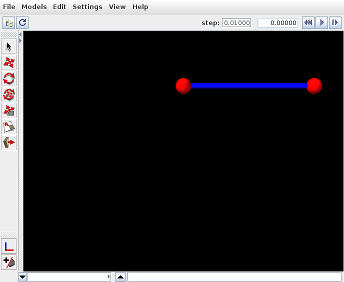
\includegraphics[width=3.75in]{images/ParticleSpring}
\end{center}
\caption{ParticleSpring example loaded into ArtiSynth.}
\label{ParticleSpring:fig}
\end{figure}

An complete application model that implements a simple particle-spring
model is given below. 
\lstset{numbers=left}
\lstinputlisting{../../src/artisynth/demos/tutorial/ParticleSpring.java}
\lstset{numbers=none}

Line 1 of the source defines the package in which the model class will
reside, in this case {\tt artisynth.demos.tutorial}. Lines 3-8 import
definitions for other classes that will be used.

The model application class is named {\tt ParticleSpring} and declared
to extend {\tt RootModel} (line 13), and the {\tt build()} method
definition begins at line 15. (A no-args constructor is also needed,
but because no other constructors are defined, an empty one is created
automatically.)

To begin, the {\tt build()} method creates a {\tt MechModel} named
{\tt "mech"}, and then adds it to the models list of the root model
using the {\tt addModel()} method (lines 18-19). Next, two particles,
{\tt p1} and {\tt p2}, are created, with masses equal to 2 and initial
positions at 0, 0, 0, and 1, 0, 0, respectively (lines 22-23). Then an
axial spring is created, with end points set to {\tt p1} and {\tt p2},
and assigned a linear material with a stiffness and damping of 20 and
10 (lines 24-27). Finally, after the particles and the spring are
created, they are added to the {\tt particles} and {\tt axialSprings}
component lists of the {\tt MechModel} using the methods {\tt
addParticle()} and {\tt addAxialSpring()} (lines 30-32).

At this point in the code, both particles are defined to be
dynamically controlled, so that running the simulation would cause
both to fall under the {\tt MechModel}'s default gravity acceleration
of $(0, 0, -9.8)$. However, for this example, we want the first
particle to remain fixed in place, so we set it to be {\it
non-dynamic} (line 34), meaning that the physical simulation will not
update its position in response to forces (Section
\ref{DynamicVsParametric:sec}).

The remaining calls control aspects of how the model is graphicaly
rendered.  {\tt setBounds()} (line 37) increases the model's "bounding
box" so that by default it will occupy a larger part of the viewer
frustum. Both {\tt setPointRenderProps()} and {\tt
setSpringRenderProps()} are convenience methods defined by the class
(lines 44-48 and 5054) to set render properties for points and
springs, respectively. Points are set to be rendered as red spheres
with a radius of 0.06, while springs are set to be rendered as blue
cylinders with a radius of 0.02. More details about setting render
properties are given in Section \ref{RenderProperties:sec}.

To run this example in ArtiSynth, select {\sf All demos > tutorial >
ParticleSpring} from the {\sf Models} menu. The model should load and
initially appear as in Figure \ref{ParticleSpring:fig}.  Running
the model (Section \ref{LoadingAndRunning:sec}) will
cause the second particle to fall and swing about under gravity.

\subsubsection{Dynamic, parameteric, and attached components}
\label{DynamicVsParametric:sec}

By default, a dynamic component is advanced through time in response
to the forces applied to it. However, it is also possible to set a
dynamic component's {\tt dynamic} property to {\tt false}, so that it
does not respond to force inputs.  As shown in the example above, this
can be done using the method
\javamethod*[artisynth.core.mechmodels.DynamicComponent]{setDynamic()}:
%
\begin{verbatim}
  comp.setDynamic (false);
\end{verbatim}
%
The method
\javamethod*[artisynth.core.mechmodels.DynamicComponent]{isDynamic()}
can be used to query the {\tt dynamic} property.

Dynamic components can also be {\tt attached} to other dynamic
components (as mentioned in Section \ref{PhysicsSimulation:sec}) so
that their positions and velocities are controlled by the {\it master}
components that they are attached to.  To attach a dynamic component,
one creates an {\tt AttachmentComponent} specifying the attachment
connection and adds it to the {\tt MechModel}, as described in Section
\ref{Attachments:sec}.  The method
\javamethod*[artisynth.core.mechmodels.DynamicComponent]{isAttached()}
can be used to determine if a component is attached, and if it is,
\javamethod*[artisynth.core.mechmodels.DynamicComponent]{getAttachment()}
can be used to find the corresponding {\tt AttachmentComponent}.

Overall, a dynamic component can be in one of three states:

\begin{description}

\item[active]\mbox{}

Component is dynamic and unattached. The method
\javamethod*[artisynth.core.mechmodels.DynamicComponent]{isActive()}
returns {\tt true}. The component will move in response to forces.

\item[parametric]\mbox{}

Component is not dynamic, and is unattached. 
The method
\javamethod*[artisynth.core.mechmodels.DynamicComponent]{isParametric()}
returns {\tt true}.
The component will either remain
fixed, or will move around in response to external inputs specifying
the component's position and/or velocity. One way to supply such
inputs is to use controllers or input probes, as described in
Section \ref{SimulationControl:sec}.

\item[attached]\mbox{}

Component is attached. The method
\javamethod*[artisynth.core.mechmodels.DynamicComponent]{isAttached()}
returns {\tt true}. The component will move so as to follow the other
component(s) to which it is attached.

\end{description}

TODO setTargetPos

\subsubsection{Custom axial materials}

Application authors may also create their
own materials by subclassing the functions
%
\begin{lstlisting}[]
  double computeF (l, ldot, l0, excitation);
  double computeDFdl (l, ldot, l0, excitation);
  double computeDFdldot (l, ldot, l0, excitation);
  boolean isDFdldotZero ();
\end{lstlisting}
%
where {\tt excitation} is an additional {\it excitation} signal $a$, which
is used to implement active springs and which in particular is used to
implement axial muscles (Section \ref{PointToPointMuscles:sec}), for
which $a$ is usually in the range $[0, 1]$.

The first three methods should return the values of 
%
\begin{equation}
f (l, \dot l, a), \quad
\frac{\partial f(l, \dot l, a)}{\partial l}, \quad \text{and} \quad
\frac{\partial f(l, \dot l, a)}{\partial \dot l},
\end{equation}
%
respectively, while the last method should return {\tt true} if
$\partial f(l, \dot l, a) / \partial \dot l \equiv 0$; i.e., if it always
equals 0.

\subsubsection{Damping parameters}

Mechanical models usually contain damping forces in addition to
spring-type restorative forces. Damping generates forces that reduce
dynamic component velocities, and is usually the major source of
energy dissipation in the model. Damping forces can be generated by
the spring components themselves, as described above.

A general damping can also be set for all particles by setting the
{\tt MechModel}'s {\tt pointDamping} property. This causes
a force
%
\begin{equation}
\f_i = -d_p \v_i
\end{equation}
%
to be applied to all particles, where $d_p$ is the value of the {\tt
pointDamping} and $\v_i$ is the particle's velocity.

{\tt pointDamping} can be set and queried using the {\tt MechModel}
methods
%
\begin{lstlisting}
  setPointDamping (double d);
  double getPointDamping();
\end{lstlisting}
%

\begin{sideblock}
In general, whenever a component has a property {\tt propX}, that
property can be set and queried in code using methods of the form
\begin{verbatim}
  setPropX (T d);
  T getPropX();
\end{verbatim}
where {\tt T} is the class type associated with the property.
\end{sideblock}

{\tt pointDamping} can also be set for particles individualy.  This
property is {\it inherited} (Section
\ref{CompositeInheritableProperties:sec}), so that if not set
explicitly, it inherits the nearest explicitly set value in an
ancestor component.

\subsection{Rigid bodies}

Rigid bodies are implemented in ArtiSynth by the class
\javaclass[artisynth.core.mechmodels]{RigidBody}, which is a dynamic
component containing a six-dimensional position and orientation state,
a corresponding velocity state, an inertia, and an optional surface
mesh.

A rigid body is associated with its own 3D spatial coordinate frame,
and is a subclass of the more general
\javaclass[artisynth.core.mechmodels]{Frame} component.
The combined position and orientation of this frame with respect to
world coordinates defines the body's {\it pose}, and the associated 6
degrees of freedom decribe its "position" state.

\subsubsection{Frame markers}
\label{FrameMarkers:sec}

\begin{figure}[t]
\begin{center}
 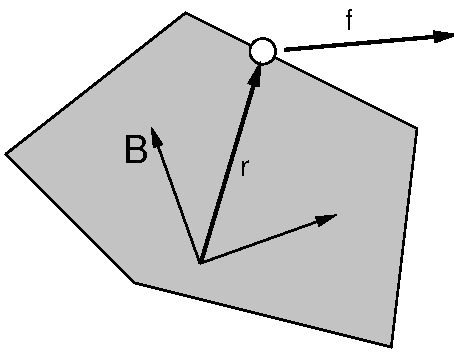
\includegraphics[width=2.5in]{images/frameMarker}
\end{center}
\caption{A force $\f$ applied to a frame marker attached to a rigid
body. The marker is located at the point $\r$ with respect to the body
coordinate frame B.}
\label{frameMarker:fig}
\end{figure}

ArtiSynth makes extensive use of {\it markers}, which are (massless)
points attached to dynamic components in the model. Markers are used
for graphical display, implementing attachments, and transmiting
forces back onto the underlying dynamic components.

A {\tt frame marker} is a marker that can be attached to a
\javaclass[artisynth.core.mechmodels]{Frame}, and most commonly to a
\javaclass[artisynth.core.mechmodels]{RigidBody} (Figure
\ref{frameMarker:fig}). They are frequently used to provide the
anchor points for attaching springs and, more generally, applying
forces to the body.

Frame markers are implemented by the class
\javaclass[artisynth.core.mechmodels]{FrameMarker}, which
is a subclass of
\javaclass[artisynth.core.mechmodels]{Point}.
The methods
%
\begin{lstlisting}
  Point3d getLocation();
  void setLocation (Point3d r);
\end{lstlisting}
%
get and set the marker's location $\r$ with respect to the frame's
coordinate system. When a 3D force $\f$ is applied to the marker, it
generates a spatial force $\hat\f$ (Section
\ref{SpatialVelocitiesAndForces:sec}) on the frame given by
%
\begin{equation}
\hat\f = \matl \f \\ \r \times \f \matr.
\end{equation}
%

\begin{figure}[h]
\begin{center}
 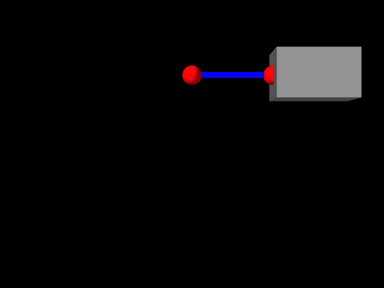
\includegraphics[width=3.75in]{images/RigidBodySpring}
\end{center}
\caption{RigidBodySpring example loaded into ArtiSynth.}
\label{RigidBodySpring:fig}
\end{figure}

\subsubsection{Example: A simple rigid body-spring model}
\label{RigidBodySpringExample:sec}

A simple rigid body-spring model is defined in
%
\begin{verbatim}
  artisynth.demos.tutorial.RigidBodySpring
\end{verbatim}
%
This differs from ParticleSpring only in the {\tt build()} method:
\lstset{numbers=left}
\begin{lstlisting}
   public void build (String[] args) {

      // create MechModel and add to RootModel
      MechModel mech = new MechModel ("mech");
      addModel (mech);

      // create the components
      Particle p1 = new Particle ("p1", /*mass=*/2, /*x,y,z=*/0, 0, 0);
      // create box and set it's pose (position/orientation):
      RigidBody box =
         RigidBody.createBox ("box", /*wx,wy,wz=*/0.5, 0.3, 0.3, /*density=*/20);
      box.setPose (new RigidTransform3d (/*x,y,z=*/0.75, 0, 0));
      // create marker point and connect it to the box:
      FrameMarker mkr = new FrameMarker (/*x,y,z=*/-0.25, 0, 0);
      mkr.setFrame (box);

      AxialSpring spring = new AxialSpring ("spr", /*restLength=*/0);
      spring.setPoints (p1, mkr);
      spring.setMaterial (
         new LinearAxialMaterial (/*stiffness=*/20, /*damping=*/10));

      // add components to the mech model
      mech.addParticle (p1);
      mech.addRigidBody (box);
      mech.addFrameMarker (mkr);
      mech.addAxialSpring (spring);

      p1.setDynamic (false);               // first particle set to be fixed

      // increase model bounding box for the viewer
      mech.setBounds (/*min=*/-1, 0, -1, /*max=*/1, 0, 0);  
      // set render properties for the components
      setPointRenderProps (p1);
      setPointRenderProps (mkr);
      setSpringRenderProps (spring);
   }
\end{lstlisting}
\lstset{numbers=none}
The differences begin at line 9. Instead of creating a second
particle, a rigid body is created using the factory method
\javamethod*[artisynth.core.mechmodels]{RigidBody.createBox()}, which
takes x, y, z widths and (uniform) density and creates a box-shaped
rigid body complete with surface mesh and appropriate mass and
inertia. As the box is initially centered at the origin, moving it
elsewhere requires setting the body's pose, which is done using {\tt
setPose()}. The {\tt RigidTransform3d} passed to {\tt setPose()} is
created using a three-argument constructor that generates a
translation-only transform.  Next, starting at line 14, a {\tt
FrameMarker} is created for a location $-0.25, 0, 0$ relative to the
rigid body, and the attached to the body using its {\tt setFrame()}
method.

The remainder of the build is the same as for ParticleSpringDemo,
except that the spring is attached to the frame marker instead of a
second particle.

To run this example in ArtiSynth, select {\sf All demos > tutorial >
RigidBodySpring} from the {\sf Models} menu. The model should load and
initially appear as in Figure \ref{RigidBodySpring:fig}.  Running the
model (Section \ref{LoadingAndRunning:sec}) will cause the rigid body
to fall and swing about under gravity.

\subsubsection{Creating rigid bodies}

As illustrated above, rigid bodies can be created using factory
methods supplied by \javaclass[artisynth.core.mechmodels]{RigidBody}.
Some of these include:
%
\begin{lstlisting}
  createBox (name, widthx, widthy, widthz, density);
  createCylinder (name, radius, height, density, nsides);
  createSphere (name, radius, density, nslices);
  createEllipsoid (name, radx, rady, radz, density, nslices);
\end{lstlisting}
%
The bodies do not need to be named; if no name is desired, then {\tt
name} and can be specified as {\tt null}.

In addition, there are also
factory methods for creating a rigid body directly from a mesh:
%
\begin{lstlisting}
  createFromMesh (name, mesh, density, scale);
  createFromMesh (name, meshFileName, density, scale);
\end{lstlisting}
%
These take either a polygonal mesh (Section \ref{Meshes:sec}), or a
file name from which a mesh is read, and use it as the body's surface
mesh and then compute the mass and inertia properties from a specified
uniform density.

Alternatively, once can create a rigid body directly from a
constructor, and then set the mesh and inertia properties explicitly:
%
\begin{lstlisting}[]
  PolygonalMesh femurMesh;
  SpatialInertia inertia;

  ... initialize mesh and inertia appropriately ...

  RigidBody body = new RigidBody ("femur");
  body.setMesh (femurMesh);
  body.setInertia (inertia);
\end{lstlisting}
%

\subsubsection{Pose and velocity}

A body's pose can be set and
queried using the methods
%
\begin{lstlisting}[]
  setPose (RigidTransform3d T);   // sets the pose to T
  getPose (RigidTransform3d T);   // gets the current pose in T
  RigidTransform3d getPose();     // returns the current pose (read-only)
\end{lstlisting}
%
These use a \javaclass[maspack.matrix]{RigidTransform3d} (Section
\ref{RigidTransform3d:sec}) to describe the pose. Body poses are
described in world coordinates and specify the transform from body to
world coordinates. In particular, the pose for a body A would specify
the rigid transform $\T_{AW}$.

Rigid bodies also expose the position and rotational components of
their pose via the properties {\tt position} and {\tt orientation},
which can be queried and set independently using the methods
%
\begin{lstlisting}[]
  setPosition (Point3d p);       // sets the position to p
  getPosition (Point3d p);       // gets the current position in p
  Point3d getPosition();         // returns the current position (read-only)

  setOrientation (AxisAngle a);  // sets the orientation to a
  getOrientation (AxisAngle a);  // gets the current orientation in a
  AxisAngle getOrientation();    // returns the current orientation (read-only)
\end{lstlisting}
%

The velocity of a rigid body is described using a
\javaclass[maspack.spatialmotion]{Twist} (Section
\ref{SpatialVectors:sec}), which contains both the translational and
rotational velocities. The methods
%
\begin{lstlisting}[]
  setVelocity (Twist v);         // sets the spatial velocity to v
  getVelocity (Twist v);         // gets the current spatial velocity in v
  Twist getVelocity();           // returns current spatial velocity (read-only)
\end{lstlisting}
%
set and query the spatial velocity as described with respect to world
coordinates.

During simulation, the pose and velocity of a rigid body are typically
updated in response to forces, so setting the pose or velocity
generally makes only for setting initial conditions.

TODO setTargetPos

\subsubsection{Inertia and meshes}

The "mass" of a rigid body is described by its spatial inertia
(Section \ref{SpatialInertia:sec}), implemented by a
\javaclass[maspack.spatialmotion]{SpatialInertia} object, which
specifies its mass, center of mass, and rotational inertia with
respect to the center of mass.

Most rigid bodies are also associated with a polygonal surface mesh,
which can be set and queried using the methods
%
\begin{lstlisting}
  setMesh (PolygonalMesh mesh);
  setMesh (PolygonalMesh mesh, String meshFileName);
  PolygonalMesh getMesh();
\end{lstlisting}
%
The second method takes an optional {\tt fileName} argument that can
be set to the name of a file from which the mesh was read. Then if the
model itself is saved to a file, the model file will specify the mesh
using the file name (instead of explicit vertex and face information),
which can reduce the model file size considerably.

The inertia of a rigid body can be explicitly set using a variety
of methods including
%
\begin{lstlisting}
  setInertia (M)		    // SpatialInertia
  setInertia (mass, Jxx, Jyy, Jzz); // mass and diagonal rotational inertia
  setInertia (mass, J);             // mass and full rotational inertia
  setInertia (mass, J, com);        // mass, rotational inertia, center-of-mass
\end{lstlisting}
%
and can be queried using 
%
\begin{lstlisting}
  getInertia (M);                   // get SpatialInertia in M
  getInertia ();                    // return read-only SpatialInertia
\end{lstlisting}
%

In practice, it is often more convenient to simply specify a mass or a
density, and then use the volume defined by the surface mesh to
compute the remaining inertial values. How a rigid body's inertia is
computed is determined by its {\tt inertiaMethod} property, which can
be one

\begin{description}

\item[Density]\mbox{}

Inertia is computed from density;

\item[Mass]\mbox{}

Inertia is computed from mass;

\item[Explicit]

Inertia is set explicitly.

\end{description}

This property can be set and queried using
%
\begin{lstlisting}
  setInertiaMethod (InertiaMethod method);
  InertiaMethod getInertiaMethod();
\end{lstlisting}
%
and it's default value is {\tt Density}. Explicitly setting the
inertia using one of the above {\tt setInertia()} methods will cause
the value to change to {\tt Explicit}. The method
%
\begin{lstlisting}
  setInertiaFromDensity (density); 
\end{lstlisting}
%
will (re)compute the inertia using the mesh and a density value
and set {\tt inertiaMethod} to {\tt Density}, and
the method
%
\begin{lstlisting}
  setInertiaFromMass (mass); 
\end{lstlisting}
%
will (re)compute the inertia using the mesh and mass value
and set {\tt inertiaMethod} to {\tt Mass}.

Finally, the (assumed uniform) density of the body can be queried
using
%
\begin{lstlisting}
   getDensity();
\end{lstlisting}
%

\subsubsection{Damping parameters}
\label{RigidBodyDamping:sec}

As with particles, it is possible to set damping parameters for rigid
bodies. 

{\tt MechModel} provides two properties, {\tt frameDamping} and {\tt
rotaryDamping}, which generate a spatial force centered on each rigid
body's coordinate frame
%
\begin{equation}
\hat\f_i = \matl -d_f \v_i \\ -d_r \Bom_i \matr,
\end{equation}
%
where $d_f$ and $d_r$ are the {\tt frameDamping} and {\tt
rotaryDamping} values, and $\v_i$ and $\Bom_i$ are the translational
and angular velocity of the body's coordinate frame.
The damping parameters can be set and queried using the {\tt MechModel}
methods
%
\begin{lstlisting}
  setFrameDamping (double df);
  setRotaryDamping (double dr);
  double getFrameDamping();
  double getRotaryDamping();
\end{lstlisting}
%

Frame and rotatary damping can also be set for individual bodies using
their own (inherited) {\tt frameDamping} and {\tt rotaryDamping}
properties.

\subsection{Joints and connectors}

In a typical mechanical model, many of the rigid bodies are
interconnected, either using spring-type components that exert binding
forces on the bodies, or through joint-type connectors that enforce
the connection using hard constraints.

\subsubsection{Joints and coordinate frames}

Consider two bodies A and B. The pose of body B with respect to body A
can be described by the 6 DOF rigid transform $\T_{BA}$.  If bodies A
and B are unconnected, that $\T_{BA}$ may assume any possible value
and has a full six degrees of freedom. A {\it joint} between A and B
restricts the set of poses that are possible between the two bodies
and reduces the degrees of freedom available to $\T_{BA}$.  For
simplicity, joints have their own coordinate frames for describing
their constraining actions, and then these frames are related to the
frames of the associated bodies by auxiliary transformations.

\begin{figure}[h]
\begin{center}
 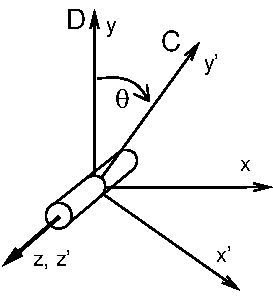
\includegraphics[width=2.5in]{images/jointExample}
\end{center}
\caption{Coordinate frames D and C for a revolute joint.}
\label{jointExample:fig}
\end{figure}

Each joint is associated with two coordinate frames C and D which move
with respect to each other as the joint moves. The allowed joint
motions therefore correspond to the allowed values of the {\it joint transform}
$\T_{CD}$.  D is the {\it base} frame and C is the {\it constraint}
frame. For a revolute joint (Figure \ref{jointExample:fig}), C can
move with respect to D by rotating about the z axis. Other motions are
prohbited. $\T_{CD}$ therefore always has the form
%
\begin{equation}
\T_{CD} = \matl
\cos(\theta) & -sin(\theta) & 0 \\
\sin(\theta) &  cos(\theta) & 0 \\
0 & 0 & 1\\
\matr
\end{equation}
%
where $\theta$ is the angle of joint rotation and is known as the {\it
joint parameter}. Other joints have different parameterizations.

\begin{figure}[h]
\begin{center}
 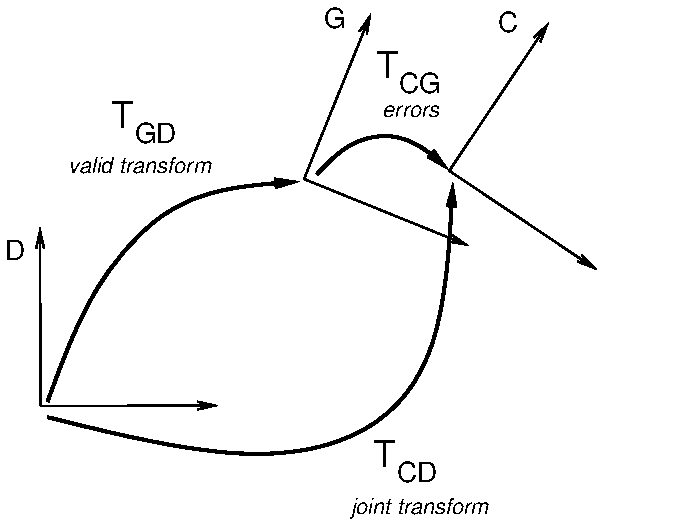
\includegraphics[width=2.5in]{images/jointFrames}
\end{center}
\caption{Schematric showing the joint base frame D, frame C that accounts for
allowed joint motion, and frame F that accounts for additional errors
and complaint motion.}
\label{jointFrames:fig}
\end{figure}

Each joint is also associated with an additional frame F that is
nominally aligned with C but which varies from C to accomodate
additional motions of the joint due to numerical error and compliance
in the joint constraints (Section \ref{JointCompliance:sec}). Frames
C, D, and F are all shown in Figure \ref{jointFrames:fig} along with
their associated transforms.  $\T_{CD}$ accounts for the nominal
allowed joint motion, $\T_{FC}$ accounts for additional motions due to
numerical error and compliance, and the overall {\it joint transform}
$\T_{FD} = \T_{CD} \, T_{FC}$ accounts for the entire joint motion.
If there is no compliance or joint error, then frames F and C are the
same, $\T_{FC} = \I$ (where $\I$ is the identity transform), and
$\T_{FD} = \T_{FC}$.  When the joint transform $\T_{FD}$ is itself
the identity, the joint is said to be in the {\it zero state}.

In general, each joint is attached to two rigid bodies A and B, with
frame F being fixed to body A and frame D being fixed to body B. The
restrictions of the joint transform $\T_{FD}$ therefore restrict the
relative poses of A and B.

\begin{figure}[h]
\begin{center}
 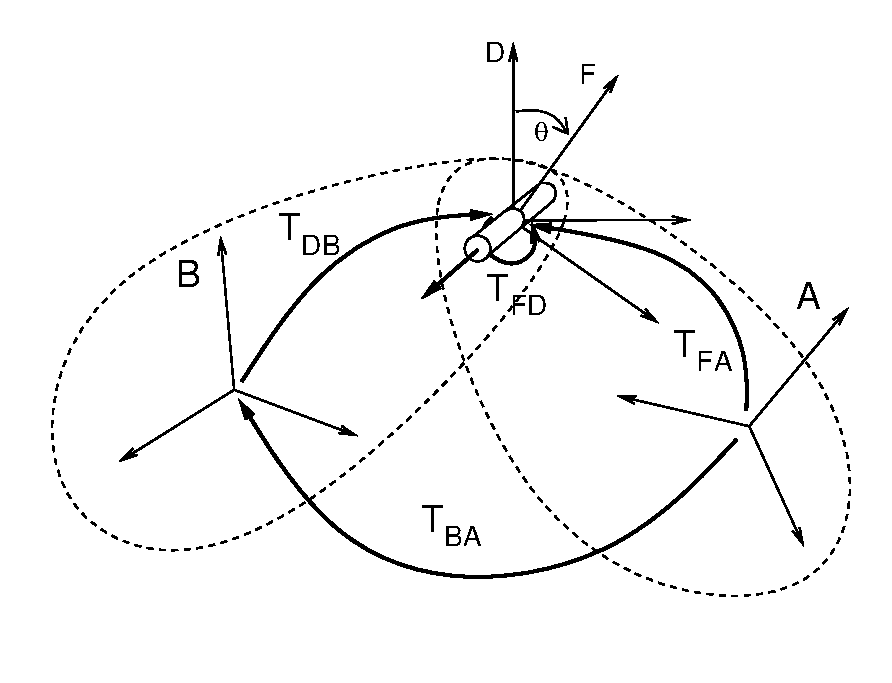
\includegraphics[width=3.74in]{images/jointBodyFrames}
\end{center}
\caption{Tranforms connecting joint coordinate frames F and D with
rigid bodies A and B. Dotted lines indicate the bodies themselves.}
\label{jointBodyFrames:fig}
\end{figure}

Except in special cases, the joint coordinate frames F and D are not
coincident with the body frames A and B.  Instead, they are located
relative to A and B by the transforms $\T_{FA}$ and $\T_{DB}$,
respectively (Figure \ref{jointBodyFrames:fig}). 
Since $\T_{FA}$ and $\T_{DFA}$ are both fixed, the pose
of B relative to A can be determined from
the joint transform $\T_{FD}$:
%
\begin{equation}
\T_{BA} = \T_{FA} \, \T_{FD}^{-1} \, \T_{DB}^{-1}.
\label{jointPose:eqn}
\end{equation}
%
(See Section \ref{RigidTransforms:sec} for a discussion of determining
transforms between related coordinate frames).

\subsubsection{Creating Joints}
\label{CreatingJoints:sec}

Joint components in ArtiSynth are implemented by subclasses of
\javaclass[artisynth.core.mechmodels]{RigidBodyConnector}.  Some of
the commonly used ones are described in Section
\ref{CommonJoints:sec}.

An application creates a joint by constructing it and adding it to a
{\tt MechModel}. Most joints generally have a constructor of the form
%
\begin{lstlisting}
  JointType (bodyA, XFA, bodyB, XDB);
\end{lstlisting}
%
which specifies the rigid bodies A and B which the joint connects,
along with the transforms $\T_{FA}$ and $\T_{DB}$. These transform
values must be set to locate the joint appropriately with respect to
the bodies. The bodies and transforms may also be set
using the method
\javamethodAlt{artisynth.core.mechmodels.RigidBodyConnector.setBodies()}
{setBodies(bodyA, XFA, bodyB, XDB)}.

A common way to determine
$\T_{FA}$ and $\T_{DB}$ is to first assume that the joint is in the
zero state (so that $\T_{FD} = \I$ and frames F and D are the same),
specify $\T_{FA}$ which then gives both F and D with respect to A,
compute $\T_{BA}$ from the world body poses $\T_{AW}$ and
$\T_{BW}$
%
\begin{equation}
\T_{BA} = \T_{AW}^-1 \; \T_{BW},
\end{equation}
%
and finally use (\ref{jointPose:eqn}) to solve for $\T_{DB}$:
%
\begin{equation}
\T_{DB} = \T_{BA}^{-1} \; \T_{FA}.
\end{equation}
%
This can be accomplished using the following code fragment:
%
\begin{lstlisting}
   RigidBody bodyA, bodyB;
   RigidTransform3d TFA = new RigidTransform3d();
   RigidTransform3d TDB = new RigidTransform3d();
	
   ... set TFA explicitly ...

   RigidTransform3d TBA = new RigidTransform3d(); // pose of B wrt A
   TBA.mulInverseLeft (bodyA.getPose(), bodyB.getPose());
   TDB.mulInverseLeft (TBA, TFA);   
\end{lstlisting}
%
If it is prefered to specify F in world coordinates, 
using $\T_{FW}$, then one can compute 
$\T_{FA}$ from $\T_{AW}$:
%
\begin{equation}
\T_{FA} = \T_{AW}^{-1} \; \T_{FW},
\end{equation}
%
which may be expressed in code as
\begin{lstlisting}
   ... set TFA explicitly to TFW ...

   // convert to TFA
   TFA.mulInverseLeft (bodyA.getPose(), TFA);
\end{lstlisting}

Sometimes when setting up a joint it may be preferable to


Alternatively, we may have




Once a joint has been created and added to a {\tt MechModel}, it is
sometimes possible to "move" it by explicitly setting its joint
parameters. This will cause the transform $\T_{CD}$ to be explicity
set to the value implied by the joint parameters, the error transform
$\T_{FC}$ to be set to the identity, and the joint transform 
$\T_{FD}$ to therefore be set to $\T_{CD}$. The position
of B relative to A is then updated using (\ref{jointPose:eqn}),
and either body A or body B is moved accr

If desired, joints can be connected to only a single rigid body. In
this case, the second body B is simply assumed to be "ground", and the
coordinate frame that would be associated with body B is instead taken
to be the world coordinate frame W. The corresponding constructor
takes the form
%
\begin{lstlisting}
  JointType (bodyA, XFA, XDW);
\end{lstlisting}
%
One may also use
\javamethodAlt{artisynth.core.mechmodels.RigidBodyConnector.setBodies()}
{setBodies(bodyA, XFA, null, XDW)}.

\subsubsection{Example:  A simple revolute joint}
\label{RigidBodyJoint:sec}

\begin{figure}[h]
\begin{center}
 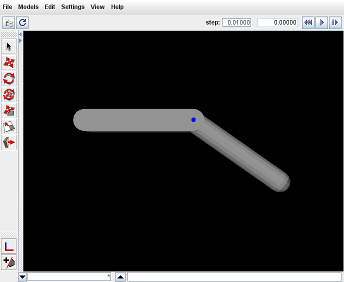
\includegraphics[width=3.75in]{images/RigidBodyJoint}
\end{center}
\caption{RigidBodyJoint example loaded into ArtiSynth.}
\label{RigidBodyJoint:fig}
\end{figure}

A simple model showing two rigid bodies connected by
a joint is defined in
%
\begin{verbatim}
  artisynth.demos.tutorial.RigidBodyJoint
\end{verbatim}
%

The build method for this model is given below:
\lstset{numbers=left}
\begin{lstlisting}
   public void build (String[] args) {

      // create MechModel and add to RootModel
      mech = new MechModel ("mech");
      mech.setGravity (0, 0, -98);
      mech.setFrameDamping (1.0);
      mech.setRotaryDamping (4.0);
      addModel (mech);

      PolygonalMesh mesh;  // bodies will be defined using a mesh

      // create first body and set its pose
      mesh = MeshFactory.createRoundedBox (lenx1, leny1, lenz1, /*nslices=*/8);
      RigidTransform3d TMB = 
         new RigidTransform3d (0, 0, 0, /*axisAng=*/1, 1, 1, 2*Math.PI/3);
      mesh.transform (TMB);
      bodyB = RigidBody.createFromMesh ("bodyB", mesh, /*density=*/0.2, 1.0);
      bodyB.setPose (new RigidTransform3d (0, 0, 1.5*lenx1, 1, 0, 0, Math.PI/2));
      bodyB.setDynamic (false);

      // create second body and set its pose
      mesh = MeshFactory.createRoundedCylinder (
         leny2/2, lenx2, /*nslices=*/16, /*nsegs=*/1, /*flatBottom=*/false);
      mesh.transform (TMB);
      bodyA = RigidBody.createFromMesh ("bodyA", mesh, 0.2, 1.0);
      bodyA.setPose (new RigidTransform3d (
                        (lenx1+lenx2)/2, 0, 1.5*lenx1, 1, 0, 0, Math.PI/2));

      // create the joint      
      RigidTransform3d TFA = new RigidTransform3d (-lenx2/2, 0, 0);
      RigidTransform3d TDB = new RigidTransform3d();
      TDB.mulInverseLeft (bodyB.getPose(), bodyA.getPose());
      TDB.mul (TFA);
      RevoluteJoint joint = new RevoluteJoint (bodyA, TFA, bodyB, TDB);

      // add components to the mech model
      mech.addRigidBody (bodyB);
      mech.addRigidBody (bodyA);
      mech.addRigidBodyConnector (joint);

      joint.setTheta (35);  // set joint position

      // set render properties for components
      joint.setAxisLength (4);
      RenderProps.setLineColor (joint, Color.BLUE);
      RenderProps.setLineRadius (joint, 0.2);
   }
\end{lstlisting}
\lstset{numbers=none}

A {\tt MechModel} is created as usual at line 4. However, in this
example, we also set some parameters for it:
\javamethod*[artisynth.core.mechmodels]{setGravity()} is used to set
the gravity acceleration vector to $(0, 0, -98)^T$ instead of the
default value of $(0, 0, -9.8)^T$, and frame and rotary damping
(Section \ref{RigidBodyDamping:sec}) are set to provide dissipation.

Each of the two rigid bodies are created from a mesh and a density.
The meshes themselves are created using the factory methods
\javamethod*[maspack.geometry]{MechFactory.createRoundedBox()} and
\javamethod*[maspack.geometry]{MechFactory.createRoundedCylinder()}
(lines 13 and 22), and then
\javamethod*[artisynth.core.mechmodels]{RigidBody.createFromMesh()} is
used to turn these into rigid bodies with a density of 0.2 (lines 17
and 25). The pose of the two bodies is set using {\tt
RigidTransform3d} objects created with x, y, z translation and
axis-angle orientation values (lines 18 and 26).

The revolute joint is implemented using
\javaclass[artisynth.core.mechmodels]{RevoluteJoint}, which is
constructed at line 34 using transform values {\tt TFA} and {\tt TDB}
computed as described in Section \ref{CreatingJoints:sec}; the only
difference is that in lines 32 and 33 the transform 
$\T_{DB}$ is computed directly from 
%
\begin{equation}
\T_{DB} = \T_{BW}^{-1} \; \T_{AW} \; \T_{FA},
\end{equation}
%
based on the relation
%
\begin{equation}
\T_{DB} = \T_{BA}^{-1} \; \T_{FA} = (\T_{AW}^{-1} \; \T_{BW})^{-1} \; \T_{FA},
\end{equation}
%
which avoids the need to explicitly compute $\T_{BA}$.


Once the joint is created at added to the {\tt MechModel}, the method
\javamethod*[artisynth.core.mechmodels.RevoluteJoint]{setTheta()} is
used to explicity set the joint parameter to 35 degrees. This will
cause the joint transform $\T_{FD}$ to be explicitly set so
that $\T_{CD}$

To run this example in ArtiSynth, select {\sf All demos > tutorial >
RigidBodySpring} from the {\sf Models} menu. The model should load and
initially appear as in Figure \ref{RigidBodyJoint:fig}.  Running the
model (Section \ref{LoadingAndRunning:sec}) will cause {\tt bodyA} to
fall and swing under gravity.

\subsubsection{Commonly used joints}
\label{CommonJoints:sec}

TODO

\subsubsection{Joint Compliance}
\label{JointCompliance:sec}

TODO 

\subsection{Frame springs}

\subsubsection{Frame spring coordinate frames}

\subsubsection{Frame materials}

\subsubsection{Example: Two bodies connected by a frame spring}

\begin{figure}[h]
\begin{center}
 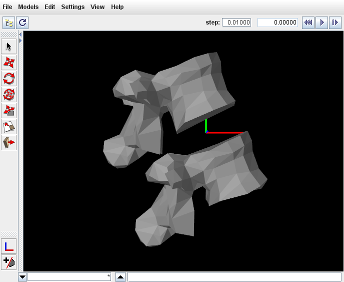
\includegraphics[width=3.75in]{images/LumbarFrameSpring}
\end{center}
\caption{LumbarFrameSpring example loaded into ArtiSynth.}
\label{LumbarFrameSpring:fig}
\end{figure}

A simple model showing two rigid bodies connected by
a frame spring is defined in
%
\begin{verbatim}
  artisynth.demos.tutorial.LumbarFrameSpring
\end{verbatim}
%

\subsection{Attachments}
\label{Attachments:sec}

\subsubsection{The attachment framework}

masters components
getMasterComponents

\subsubsection{Attaching a particle to a Frame}

\subsection{Simulation control properties}

\section{Mechanical Models II}
\label{MechModelsII:sec}

\subsection{Units}

\subsection{Multi-point springs}

\subsubsection{Operation}

\subsubsection{Example: A single multi-point spring}

\begin{figure}[h]
\begin{center}
 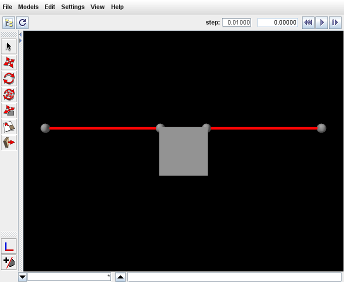
\includegraphics[width=3.75in]{images/MultiPointSpring}
\end{center}
\caption{MultiPointSpring example loaded into ArtiSynth.}
\label{MultiPointSpring:fig}
\end{figure}

A simple model showing a multi-point spring is defined in
%
\begin{verbatim}
  artisynth.demos.tutorial.MultiPointSpring
\end{verbatim}
%

% MultiPointSpring

\subsection{Point-to-point muscles}
\label{PointToPointMuscles:sec}

\subsubsection{Muscle materials}

\subsubsection{Example: Muscle attached to a rigid body}

\begin{figure}[h]
\begin{center}
 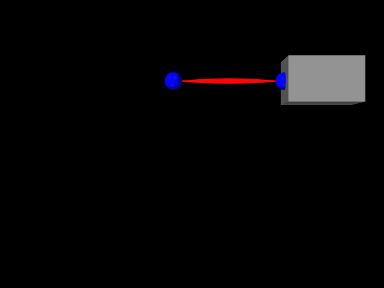
\includegraphics[width=3.75in]{images/SimpleMuscle}
\end{center}
\caption{SimpleMuscle example loaded into ArtiSynth.}
\label{SimpleMuscle:fig}
\end{figure}

A simple model showing a single muscle connected to a rigid
body is defined in
%
\begin{verbatim}
  artisynth.demos.tutorial.SimpleMuscle
\end{verbatim}
%

% SimpleMuscle

\subsubsection{Multi-point muscles}



\subsection{Mesh components}

\subsubsection{Fixed meshes}

\subsubsection{Simple mesh example}

% SimpleMesh

\subsubsection{Skinned meshes}

\subsubsection{Simple skinned mesh example}

% SimpleSkinnedMesh

\subsection{Collision Handling}

\subsubsection{Collidable bodies}

\subsubsection{Enabling collisions in code}

\subsubsection{Example: Collision with a plane}

\begin{figure}[h]
\begin{center}
 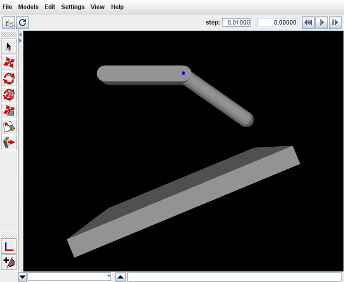
\includegraphics[width=3.75in]{images/JointedCollide}
\end{center}
\caption{JointedCollide example loaded into ArtiSynth.}
\label{JointedCollide:fig}
\end{figure}

A simple model illustrating collision between two jointed rigid bodies
and a plane is defined in
%
\begin{verbatim}
  artisynth.demos.tutorial.JointedCollide
\end{verbatim}
%

% JointedCollide

\subsubsection{implementation and limitations}

%\subsection{Moving non-dynamic components}

\subsection{General component arrangements}
\label{GeneralArrangements:sec}

\subsubsection{Component lists}

\subsubsection{General arrangement example}

% NetDemo

\subsubsection{Legacy containers in MechModel}

\subsection{Render properties}
\label{RenderProperties:sec}

\subsubsection{Render property taxonomy}

\subsubsection{Setting render properties}

\subsection{Scaling and transforming}

\subsubsection{The ScalableUnits interface}

\subsubsection{The TransformableGeometry interface}

\section{Simulation Control}
\label{SimulationControl:sec}

\subsection{Control Panels}

\subsubsection{General principles}

\subsubsection{Creating a simple control panel}

% SimpleMuscleWithPanel

\subsection{Custom properties}
\label{CustomProperties:sec}

\subsubsection{Adding custom properties to a RootModel}

\subsubsection{Example: a visibility property}

% SimpleMuscleWithProperties

\subsection{Controllers and monitors}

\subsubsection{Purpose and operation}

\subsubsection{A controller to move a point}

% SimpleMuscleWithController

\subsection{Probes}

\subsubsection{Input and output probes}

\subsubsection{Adding probes in code}

% SimpleMuscleWithProbes

\subsubsection{Probe data files}

\subsubsection{Adding probe data in-line}

\section{Finite Element Models}
\label{FEMModels:sec}

\subsection{Overview}

\subsubsection{Structure}

\subsubsection{Materials}

\subsubsection{Boundary conditions}

\subsection{FEM model creation}

\subsubsection{Using factory methods}

\subsubsection{Using external meshes}

\subsubsection{Using direct code}

\subsubsection{A simple beam model}

% FemBeam

\subsection{FEM Geometry}

\subsubsection{Surface meshes}

\subsubsection{Embedding geometry within an FEM}

\subsubsection{A beam with an embedded sphere}

% EmbeddedFemSphere

\subsection{Node attachments}

\subsubsection{General principles}

\subsubsection{Connecting a beam to a block}

% FemBeamWithBlock

\subsubsection{Connecting two FEMs together}

% ConnectedFems

\subsection{FEM markers}

\subsubsection{Embedding particles in FEMs}

\subsubsection{Attaching a FEM beam to a muscle}

% FemBeamWithMuscle

\subsection{Muscle activated FEM models}

\subsubsection{FemMuscleModel}

\subsubsection{Activation with fibres}

\subsubsection{Activation with embedded materials}

\subsubsection{Comparision with two beam examples}

% FemMuscleBeams

\subsection{Collisions}

\subsubsection{Colliding with FEM geometry}

\subsubsection{Colliding with the surface mesh}

% FemMuscleHeart

\subsubsection{Colliding with an embedded sphere}

% EmbeddedFemSphere

\subsection{Visualization}

stuff stuff stuff

\subsubsection{Rendering settings}

stuff stuff stuff

\subsubsection{Stress and strain plotting}

stuff stuff stuff

\section{Appendices}

\subsection{Appendix A: Rotation transforms}
\label{Rotations:sec}

This section reviews 3D rotation matrices and transformations.

\begin{figure}[t]
\begin{center}
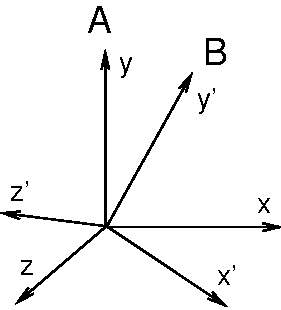
\includegraphics[width=2in]{images/rotationAB}
\end{center}
\caption{Two coordinate frames A and B rotated with respect
to each other.}
\label{rotationAB:fig}
\end{figure}

Consider two 3D coordinate frames A and B that are rotated with
respect to each other (Figure \ref{rotationAB:fig}).  The orientation
of B with respect to A can be described by a $3 \times 3$ rotation
matrix $\R_{BA}$, whose columns are the unit vectors giving the
directions of the rotated axes $\x'$, $\y'$, and $\z'$ of B with
respect to A.

$\R_{BA}$ is an {\it orthogonal} matrix, meaning that
its columns are both perpendicular and mutually
orthogonal, so that
%
\begin{equation}
\R_{BA}^T \, \R_{BA} = \I
\end{equation}
%
where $\I$ is the $3 \times 3$ identity matrix. The inverse
of $\R_{BA}$ is hence equal to its transpose:
%
\begin{equation}
\R_{BA}^{_1} = \R_{BA}^T
\label{RABinv:eqn}
\end{equation}
%
Because $\R_{BA}$ is orthogonal, $|\det \R_{BA}| = 1$, and because it
is a rotation, $\det \R_{BA} = 1$. The other case, where $\det \R_{BA}
= -1$, is not a rotation but a {\it reflection}.
The 6 orthogonality constraints associated with a rotation matrix mean
that in spite of having 9 numbers, the matrix only has 3 degrees of
freedom.

Now, assume we have a 3D vector $\v$, and consider its coordinates
with respect to both frames A and B.  Where necessary, we use a
preceding superscript to indicate the coordinate frame with repect to
which a quantity is described, so that ${}^A\v$ and ${}^B\v$ and
denote $\v$ with respect to frames A and B, respectively.  Given the
definition of $\R_{AB}$ given above, it is fairly straightforward to
show that
%
\begin{equation}
{}^A\v = \R_{BA} \, {}^B\v
\label{vectorTransform:eqn}
\end{equation}
%
and, given (\ref{RABinv:eqn}), that
%
\begin{equation}
{}^B\v = \R_{BA}^T \, {}^A\v.
\label{vectorInvTransform:eqn}
\end{equation}
%
Hence in addition to describing the orientation of B with respect to A,
$\R_{BA}$ is also a transformation matrix that maps vectors in B
to vectors in A.

It is straightforward to show that
%
\begin{equation}
\R_{BA}^{-1} = \R_{BA}^T = \R_{AB}.
\label{rotationInverse:eqn}
\end{equation}
%

\begin{figure}[t]
\begin{center}
 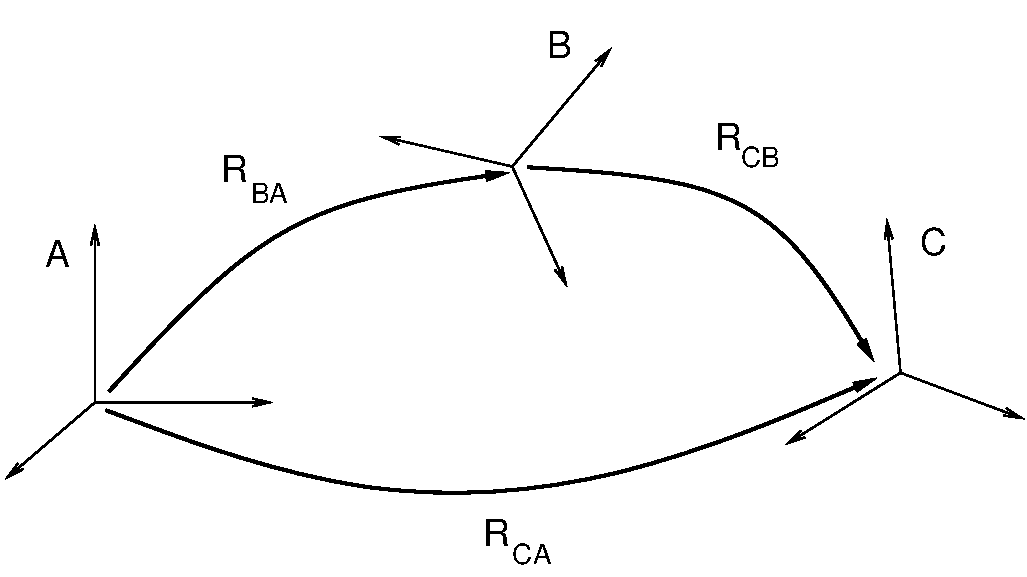
\includegraphics[width=4.5in]{images/rotationsABC}
\end{center}
\caption{Schematic illustration of three coordinate frames A, B, and C
and the rotational transforms relating them.}
\label{rotationsABC:fig}
\end{figure}

A simple rotation by an angle $\theta$ about one of the basic
coordinate axes known as a {\it basic} rotation. The three
basic rotations about x, y, and z are:
%
\begin{equation*}
\R_x(\theta) = \matl 1 & 0 & 0 \\ 
               0 & \cos(\theta) & -\sin(\theta) \\ 
               0 & \sin(\theta) & \cos(\theta) 
		 \matr
\end{equation*}
%
\begin{equation*}
\R_y(\theta) = \matl \cos(\theta) & 0 & \sin(\theta) \\ 
               0 & 1 & 0 \\ 
               -\sin(\theta) & 0 & \cos(\theta) 
                 \matr
\end{equation*}
%
\begin{equation*}
\R_z(\theta) = \matl \cos(\theta) & -\sin(\theta) & \\ 
               \sin(\theta) & \cos(theta) & 0 \\ 
               0 & 0 & 1 
                 \matr
\label{elementaryRotations:sec}
\end{equation*}
%

Next, we consider transform composition. Suppose we have three
coordinate frames, A, B, and C, whose orientation are related to each other by
$\R_{BA}$, $\R_{CB}$, and $\R_{CA}$ (Figure
\ref{transformsABC:fig}).  If we know $\R_{BA}$ and $\R_{CA}$,
then we can determine $\R_{CB}$ from
%
\begin{equation}
\R_{CB} = \R_{BA}^{-1} \, \R_{CA}.
\label{rotationCB:eqn}
\end{equation}
%
This can be understood in terms of vector transforms. $\R_{CB}$
transforms a vector from C to B, which is equivalent to first
transforming from C to A,
%
\begin{equation}
{}^A\v = \R_{CA} \, {}^C\v,
\end{equation}
%
and then transforming from A to B:
%
\begin{equation}
{}^B\v = \R_{BA}^{-1} \, {}^A\v = \R_{BA}^{-1} \; \R_{CA} {}^C\v = \R_{CB} \, {}^C\v.
\end{equation}
%
Note also from (\ref{rotationInverse:eqn}) that $\R_{CB}$ can be 
expressed as
%
\begin{equation}
\R_{CB} = \R_{AB} \, \R_{CA}.
\label{rotationCBII:eqn}
\end{equation}
%

In addition to specifying rotation matrix components explicity,
there are numerous other ways to describe a rotation.
Three of the most common are:

\begin{description}

\item[Roll-pitch-yaw angles]\mbox{}

There are 6 variations of roll-pitch-yaw angles. The one used in
ArtiSynth corresponds to older robotics texts (e.g., Paul, Spong) and
consists of a roll rotation $r$ about the z axis, followed by a pitch
rotation $p$ about the new y axis, followed by a yaw rotation $y$
about the new x axis. The net rotation can be expressed by the
following product of basic rotations: $\R_z(r) \, \R_y(p) \, \R_x(y)$.

\item[Axis-angle]\mbox{}

An axis angle rotation parameterizes a rotation as a rotation by
an angle $\theta$ about a specific axis $\u$. Any rotation
can be represented in such a way as a consequence of Euler's rotation
theorem.

\item[Euler angles]\mbox{}

There are 6 variations of Euler angles. The one used in ArtiSynth
consists of a rotation $\phi$ about the z axis, followed by a rotation
$\theta$ about the new y axis, followed by a rotation $\psi$ about the
new z axis. The net rotation can be expressed by the following product
of basic rotations: $\R_z(\phi) \, \R_y(\theta) \, \R_z(\psi)$.

\end{description}

\subsection{Appendix B: Rigid transforms}
\label{RigidTransforms:sec}

Rigid transforms are used to specify both the transformation of points
and vectors between coordinate frames, as well as the relative
position and orientation between coordinate frames.

\begin{figure}[h]
\begin{center}
 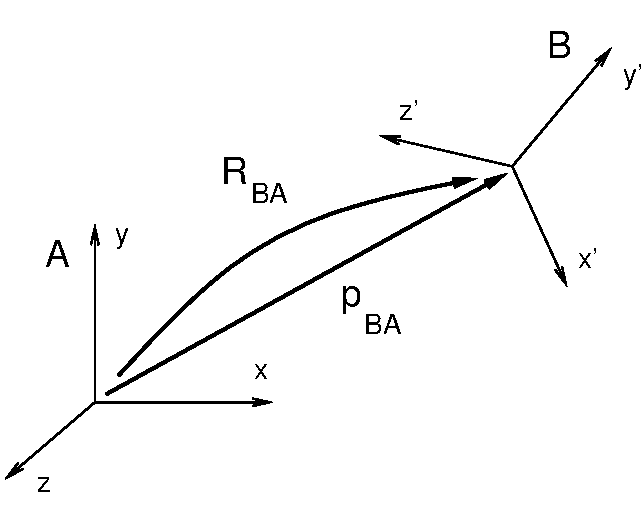
\includegraphics[width=3.25in]{images/framesAB}
\end{center}
\caption{A position vector $\p_{BA}$ and rotation matrix
$\R_{BA}$ describing the position and orientation of frame B
with respect to frame A.}
\label{framesAB:fig}
\end{figure}

Consider two 3D coordinate frames in space, A and B (Figure
\ref{framesAB:fig}). The translational position of B with respect to A
can be described by a vector $\p_{BA}$ from the origin of A to the
origin of B (described with respect to frame A). Meanwhile, the
orientation of B with respect to A can be described by the $3 \times
3$ rotation matrix $\R_{BA}$ (Section \ref{Rotations:sec}).  The
combined position and orientation of B with respect to A is known as
the {\it pose} of B with respect to A.

\begin{figure}[t]
\begin{center}
 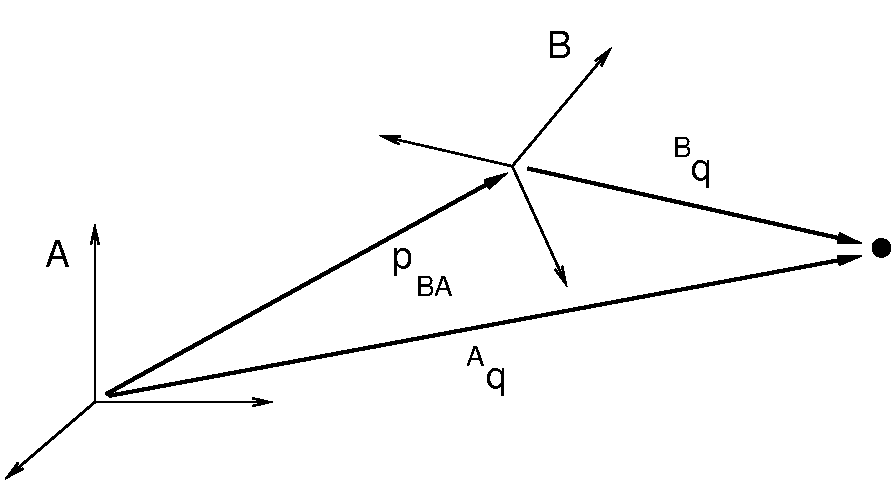
\includegraphics[width=3.75in]{images/pointsAB}
\end{center}
\caption{Point vectors ${}^A\q$ and ${}^B\q$ describing
the position of a point $\q$ with respect to frames A and B.}
\label{pointsAB:fig}
\end{figure}

Now, assume we have a 3D point $\q$, and consider its coordinates with
respect to both frames A and B (Figure \ref{pointsAB:fig}). Given the
pose descriptions given above, it is fairly straightforward to show
that
%
\begin{equation}
{}^A\q = \R_{BA} \, {}^B\q + \p_{BA}
\label{pointTransform:eqn}
\end{equation}
%
and, given (\ref{RABinv:eqn}), that
%
\begin{equation}
{}^B\q = \R_{BA}^T \, ({}^A\q - \p_{BA}).
\label{pointInvTransform:eqn}
\end{equation}
%

If we extend our points into a 4D {\it homogeneous} coordinate space
with the fourth coordinate $w$ equal to 1, i.e.,
%
\begin{equation}
\q^* \equiv \matl \q \\ 1 \matr,
\end{equation}
%
then (\ref{pointTransform:eqn}) and
(\ref{pointInvTransform:eqn}) can be simplified to
%
\begin{equation*}
{}^A\q^* = \T_{BA} \, {}^B\q^* \quad \text{and} \quad
{}^B\q^* = \T_{BA}^{-1} \, {}^A\q^*
\end{equation*}
%
where
%
\begin{equation}
\T_{BA} = \matl \R_{BA} & \p_{BA} \\ 0 & 1 \matr
\end{equation}
%
and
%
\begin{equation}
\T_{BA}^{-1} = \matl \R_{BA}^T & -\R_{BA}^T \p_{BA} \\ 0 & 1 \matr.
\end{equation}
%
$\T_{BA}$ is the $4 \times 4$ {\it rigid transform matrix} that
transforms points from B to A and also describes the pose of
B with respect to A (Figure \ref{transformAB:fig}).

\begin{figure}[t]
\begin{center}
 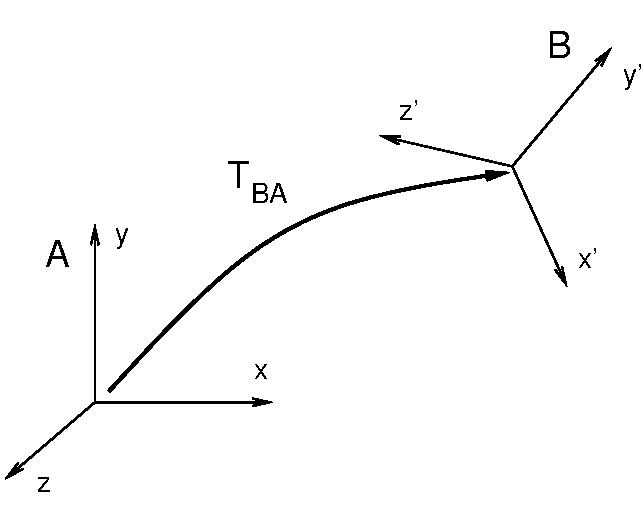
\includegraphics[width=3in]{images/transformAB}
\end{center}
\caption{The transform matrix $\T_{BA}$ from B to A.}
\label{transformAB:fig}
\end{figure}

It is straightforward to show that $\R_{BA}^T$ and $-\R_{BA}^T
\p_{BA}$ describe the orientation and position of $A$ with respect to
$B$, and so therefore
%
\begin{equation}
\T_{BA}^{-1} = \T_{AB}.
\label{transformInverse:eqn}
\end{equation}
%

Note that if we are transforming a vector $\v$ instead of a point
between B and A, then we are only concerned about relative orientation
and the vector transforms (\ref{vectorTransform:eqn}) and
(\ref{vectorInvTransform:eqn}) should be used instead.
However, we can express these using $\T_{BA}$ if
we embed vectors in a homogeneous coordinate space 
with the fourth coordinate $w$ equal to 0, i.e.,
%
\begin{equation}
\v^* \equiv \matl \v \\ 0 \matr,
\end{equation}
%
so that
%
\begin{equation*}
{}^B\v^* = \T_{BA} \, {}^A\v^* \quad \text{and} \quad
{}^A\v^* = \T_{BA}^T \, {}^B\v^*.
\end{equation*}
%

\begin{figure}[t]
\begin{center}
 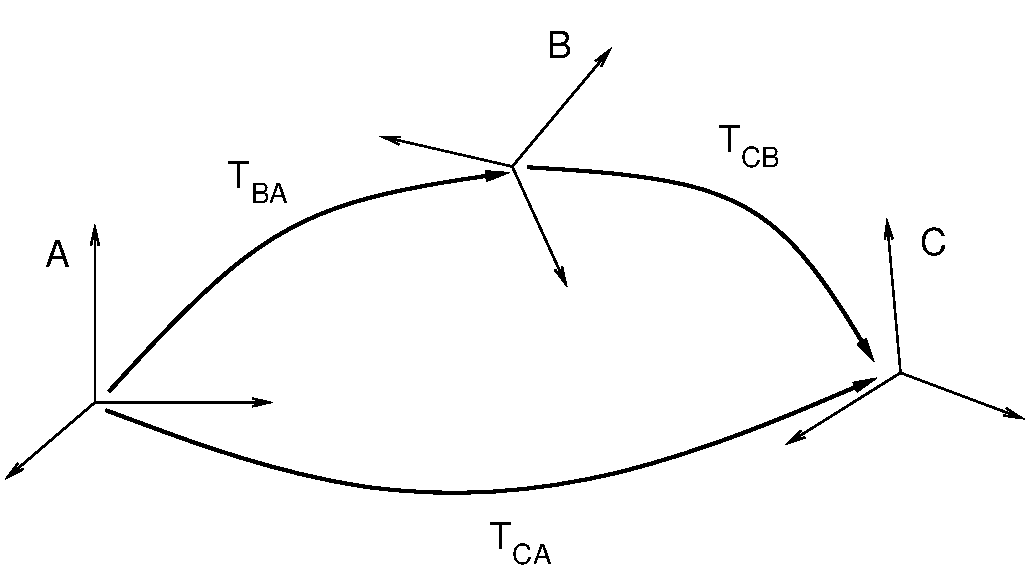
\includegraphics[width=4.5in]{images/transformABC}
\end{center}
\caption{Three coordinate frames A, B, and C and the transforms
relating each one to the other.}
\label{transformsABC:fig}
\end{figure}

Finally, we consider transform composition. Suppose we have three
coordinate frames, A, B, and C, each related to the other by
transforms $\T_{BA}$, $\T_{CB}$, and $\T_{CA}$ (Figure
\ref{transformsABC:fig}).  Using the same reasoning used to derive
(\ref{rotationCB:eqn}) and (\ref{rotationCBII:eqn}), it is easy to
show that
%
\begin{equation}
\T_{CB} = \T_{BA}^{-1} \; \T_{CA} = \T_{AB} \; \T_{CA}.
\end{equation}
%

\subsection{Appendix C: Affine transforms}
\label{AffineTransforms:sec}

An {\it affine transform} is a generalization of a rigid transform, in
which the rotational component $\R$ is replaced by a general $3 \times
3$ matrix $\A$. This means that an affine transform implements a
generalized basis transformation combined with an offset of the origin
(Figure \ref{affineAB:fig}). As with $\R$ for rigid transforms, the
columns of $\A$ still describe the transformed basis vectors $\x'$,
$\y'$, and $\z'$, but these are no longer guaranteed to orthonormal.

\begin{figure}[h]
\begin{center}
 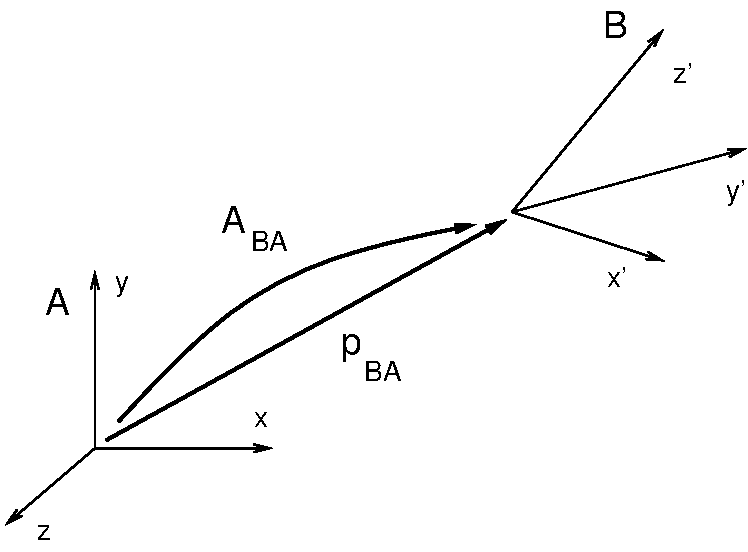
\includegraphics[width=3.25in]{images/affineAB}
\end{center}
\caption{A position vector $\p_{BA}$ and a general matrix $\A_{BA}$
describing the position and basis transform of frame B with respect to
frame A.}
\label{affineAB:fig}
\end{figure}

Expressed in terms of homogeneous coordinates,
the affine transform $\X_{AB}$ takes the form
%
\begin{equation}
\X_{BA} = \matl \A_{BA} & \p_{BA} \\ 0 & 1 \matr
\end{equation}
%
with
%
\begin{equation}
\X_{BA}^{-1} = \matl \A_{BA}^{-1} & -\A_{BA}^{\-1} \p_{BA} \\ 0 & 1 \matr.
\end{equation}
%
As with rigid transforms, when an affine transform is applied to a
vector instead of a point, only the matrix $\A$ is applied and the
translation component $\p$ is ignored.

Affine transforms are typically used to effect transformations that
require stretching and shearing of a coordinate frame.  By the polar
decomposition theorem, $\A$ can be factored into a regular
rotation $\R$ plus a symmetric shearing/scaling matrix $\P$:
%
\begin{equation}
\A = \R \, \P
\end{equation}
%
Affine transforms can also be used to perform reflections, in which
$\A$ is orthogonal (so that $\A^T \, \A = \I$) but with $\det \A =
-1$.

\subsection{Appendix D: Rotational velocity}

\begin{figure}[h]
\begin{center}
 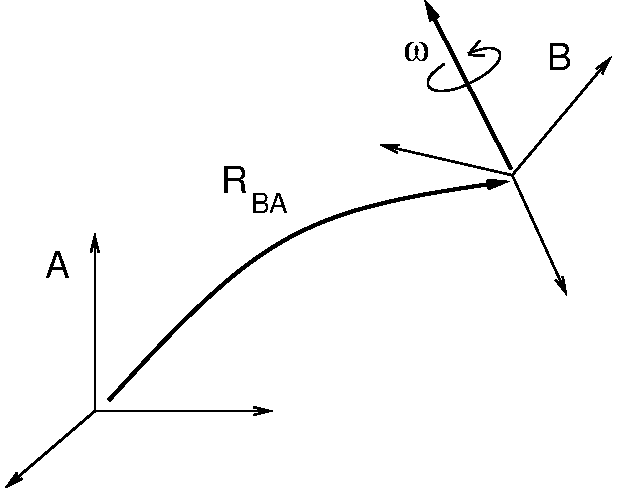
\includegraphics[width=3.25in]{images/angularvelAB}
\end{center}
\caption{Frame B rotating with respect to frame A.}
\label{angularvelAB:fig}
\end{figure}

Given two 3D coordinate frames A and B, the rotational, or {\it
angular}, velocity of B with respect to A is given by a 3D vector
$\Bom_{BA}$ (Figure \ref{angularvelAB:fig}). $\Bom_{BA}$
is related to the derivative of $\R_{BA}$ by
%
\begin{equation}
\dot\R_{BA} = [{}^A\Bom_{BA}] \R_{BA} = \R_{BA} [{}^B\Bom_{BA}]
\end{equation}
%
where ${}^A\Bom_{BA}$ and ${}^B\Bom_{BA}$ indicate $\Bom_{BA}$ with
respect to frames $A$ and $B$ and $[ \Bom ]$ denotes the $3 \times 3$
cross product matrix
%
\begin{equation}
[ \Bom ] \equiv 
\matl
0 & -\omega_z & \omega_y \\
\omega_z & 0 & -\omega_x \\
-\omega_y & \omega_x & 0 \\
\matr.
\label{xprodmatrix:eqn}
\end{equation}
%

If we consider instead the velocity of $A$ with respect to $B$, it is
straightforward to show that
%
\begin{equation}
\Bom_{AB} = -\Bom_{BA}. 
\end{equation}
%

\subsection{Appendix E: Spatial velocities and forces}
\label{SpatialVelocitiesAndForces:sec}

Given two 3D coordinate frames A and B, the {\it spatial velocity},
or {\it twist},
$\hat\v_{BA}$ of B with respect to A is given by the 6D 
composition of the translational velocity $\v_{BA}$ of the
origin of B with respect to A and the angular velocity $\Bom_{BA}$:
%
\begin{equation}
\hat\v_{BA} \equiv \matl \v_{BA} \\ \Bom_{BA} \matr.
\end{equation}
%
Similarly, the {\it spatial force}, or {\it wrench}, $\hat\f$ acting
on a frame B is given by the 6D composition of the translational force
$\f_B$ acting on the frame's origin and the moment $\Btau$, or torque,
acting through the frame's origin:
%
\begin{equation}
\hat\f_B \equiv \matl \f_B \\ \Btau_B \matr.
\end{equation}
%

\begin{figure}[h]
\begin{center}
 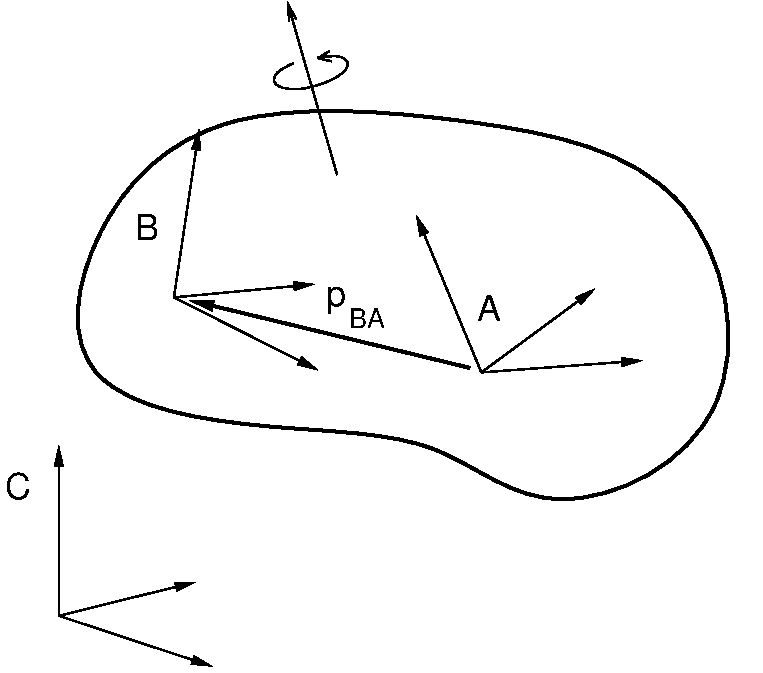
\includegraphics[width=3.25in]{images/rigidAB}
\end{center}
\caption{Two frames A and B rigidly connected within a rigid body
and moving with respect to a third frame C.}
\label{rigidAB:fig}
\end{figure}

If we have two frames $A$ and $B$ rigidly connected within a rigid
body (Figure \ref{rigidAB:fig}), and we know the spatial velocity
$\hat\v_{BC}$ of $B$ with respect to some third frame $C$, we may wish
to know the spatial velocity $\hat\v_{AC}$ of $A$ with respect to some
third frame $C$.  The angular velocity components are the same, but
the translational velocity components are coupled by the angular
velocity and the offset $\p_{BA}$ between $A$ and $B$, so that
%
\begin{equation*}
\v_{AC} = \v_{BC} - \p_{BA} \times \Bom_{BC}.
\end{equation*}
%
$\hat\v_{AC}$ is hence related to $\hat\v_{BC}$ via
\begin{equation*}
\matl \v_{AC} \\ \Bom_{AC} \matr =
\matl \I & -[\p_{BA}] \\ 0 & \I \matr \,
\matl \v_{BC} \\ \Bom_{BC} \matr.
\end{equation*}
%
where $[\p_{BA}]$ is defined by
(\ref{xprodmatrix:eqn}).

The above equation assumes that all quantities are expressed
with respect to the same coordinate frame.
If we instead consider $\hat\v_{AC}$ and $\hat\v_{BC}$ to be represented
in frames $A$ and $B$, respectively, then
we can show that
%
\begin{equation}
{}^A\hat\v_{AC} = \X_{BA} \, {}^B\hat\v_{BC},
\end{equation}
%
where
%
\begin{equation}
\X_{BA} \equiv
\matl \R_{BA} & -[\p_{BA}] \R_{BA} \\ 0 & \R_{BA} \matr.
\label{XvelAB:eqn}
\end{equation}
%
The transform $\X_{BA}$ is easily formed from the components of the
rigid transform $\T_{BA}$ relating $B$ to $A$.

The spatial forces $\hat\f_A$ and $\hat\f_B$ acting on frames $A$ and
$B$ within a rigid body are related in a similar way, only with
spatial forces, it is the moment that is coupled through the moment
arm created by $\p_{BA}$, so that
%
\begin{equation*}
\Btau_{A} = \Btau_{B} + \p_{BA} \times \f_{B}.
\end{equation*}
%
If we again assume that $\hat\f_A$ and $\hat\f_B$
are expressed in frames $A$ and $B$, we can show that
%
\begin{equation}
{}^A\hat\f_A = \X^*_{BA} \, {}^B\hat\f_B,
\end{equation}
%
where
%
\begin{equation}
\X^*_{BA} \equiv
\matl \R_{BA} & 0 \\  [\p_{BA}] \R_{BA} & \R_{BA} \matr.
\label{XforceAB:eqn}
\end{equation}
%

\subsection{Appendix F: Spatial inertia}
\label{SpatialInertia:sec}

Assume we have a rigid body with mass $m$ and a coordinate frame
located at the body's center of mass.  If $\v$ and $\Bom$ give the
translational and rotational velocity of the coordinate frame, then
the body's linear and angular momentum $\p$ and $\L$ are given by
%
\begin{equation}
\p = m \v \quad \text{and} \quad \L = \J \Bom,
\label{momenta:eqn}
\end{equation}
%
where $\J$ is the $3 \times 3$ {\it rotational inertia} with respect
to the center of mass. These relationships can be combined into a
single equation
%
\begin{equation}
\hat\p = \M \hat\v,
\label{momentum:eqn}
\end{equation}
%
where $\hat\p$ and $\M$ are the {\it spatial momentum} and
{\it spatial inertia}:
%
\begin{equation}
\hat\p \equiv \matl \p \\ \L \matr, \qquad
\M \equiv \matl m \I & 0 \\ 0 & \J \matr.
\end{equation}
%
The spatial momentum satisfies Newton's second law, so that
%
\begin{equation}
\hat\f = \frac{d \hat\p}{dt} = \M \frac{d \hat\v}{dt} + \dot\M \hat\v,
\end{equation}
%
which can be used to find the acceleration of a body in response to a
spatial force.

When the body coordinate frame is {\it not} located at the center of
mass, then the spatial inertia assumes the more complicated form
%
\begin{equation}
\matl 
m \I & -m [\c] \\ m [\c] & \J - m[\c][\c]
\matr,
\end{equation}
%
where $\c$ is the center of mass and $[\c]$ is defined by
(\ref{xprodmatrix:eqn}).

\iflatexml
\bibliographystyle{plain}
\bibliography{references}
\else
\bibliographystyle{plain}
\begin{btSect}{references}
\btPrintCited
\end{btSect}
\fi

\end{document}
